% 全国大学生数学建模竞赛论文 —— 基于光滑化策略与梯度类算法的信号重构问题研究
% 编译: xelatex main.tex (两次)
\documentclass[withoutpreface,bwprint]{cumcmthesis}
\usepackage{cumcm2026}
\usepackage{subcaption}
\usepackage{booktabs}
\usepackage{bm}
\usepackage{multirow}

% 附录代码样式：无底色、无行号的简洁代码块
\lstdefinestyle{appcode}{
  basicstyle=\ttfamily\scriptsize,
  frame=single,
  rulecolor=\color{black!30},
  breaklines=true,
  breakatwhitespace=false,
  showstringspaces=false,
  columns=fullflexible,
  keepspaces=true
}

% 三线表伪代码环境（仿优秀论文 Algorithm 样式）
\newenvironment{algtable}[1]{%
  \par\medskip\noindent
  \begin{minipage}{\textwidth}\scriptsize
  \begin{tabular}{p{\dimexpr\textwidth-2\tabcolsep}}
    \toprule
    \textbf{#1} \\
    \midrule
}{%
    \\ \bottomrule
  \end{tabular}
  \end{minipage}
  \par\medskip
}

\title{基于光滑化策略与梯度类算法的信号重构问题研究}

%% 封面信息
\tihao{A}
\baominghao{}
\schoolname{}
\membera{}
\memberb{}
\memberc{}
\supervisor{}
\yearinput{2026}
\monthinput{9}
\dayinput{1}

\begin{document}

\maketitle

\begin{abstract}
信号重构是信号处理的核心问题：图像在采集与传输中常被椒盐噪声污染，压缩感知中
需要由少量线性观测恢复高维稀疏信号，二者在数学上均可归结为带 $\ell_1$ 型非光滑
项的凸优化模型，其求解质量取决于模型的建立与数值算法的设计。本文围绕
``非光滑问题的光滑化处理、凸模型的盒约束化、投影梯度与共轭梯度两类算法设计''
这一主线，对三个问题建立统一的建模求解框架，并给出完整的数值检验。

针对问题一，首先，按``取值为动态范围端点且被滤波器替换''的两条件定义确定噪声
候选集，将误检率控制在 $1\%$ 以内；其次，在候选集上建立含 $\ell_1$ 数据保真项与
保边正则项的凸泛函，利用势函数的偶对称性将正则项改写为仅依赖四邻域查值的边和
形式；再次，以平方根型光滑函数逼近绝对值函数，并由最大值原理把模型约束到像素
动态范围，得到盒约束光滑凸问题；最后，设计 BB 步长的投影梯度算法求解。在
12 张标准测试图、2 个噪声等级、3 组随机种子共 72 个算例上全部收敛，平均恢复
PSNR 为 37.33 dB 与 33.76 dB；Lena 图在 30\% 噪声下达到 38.35 dB，
较自适应中值滤波直接输出提高 4.47 dB。

针对问题二，将五种保边势函数置于同一恢复框架下，先逐一分析其光滑性、导数
有界性与原点曲率等解析性质，再按``各自独立标定参数、统一条件下做参数迁移验证''
的协议比较。结果表明：各势函数在标定参数下恢复质量接近（PSNR 极差 0.19 dB 与
0.13 dB），差异主要体现在参数敏感性与收敛速度。平方根型的参数平台较宽且
收敛最快；光滑化幂函数型的恢复质量与效率也较稳定；对数余弦型、对数型和
Huber 型在本文求解配置下需要更多迭代。据此优先推荐平方根型或光滑化幂函数型。

针对问题三，将光滑化策略迁移到 $\ell_1$ 正则化最小二乘，配合光滑参数逐级续延，
用修正 PRP 共轭梯度法（强 Wolfe 线搜索与下降性重启）求解，并与变量分裂框架下的
GPSR-BB 投影梯度法在完全一致的实例上对比。在 4096 维、160 尖峰实例上，
两法均完整恢复全部非零元；按``同目标值''口径修正 PRP 的迭代数为 GPSR 的 4.2 倍，
去偏置后相对误差 0.0286 对 0.0265，恢复质量基本持平；共轭参数对照显示修正 PRP
与 HS 参数的迭代数不到 FR 与 DY 参数的四分之一。

\cumcmkeywords{两阶段图像恢复；$\ell_1$ 光滑化；保边势函数；投影梯度算法；共轭梯度法}
\end{abstract}

%目录不需要
%\tableofcontents

\section{问题重述}

\subsection{问题背景}

信号处理是一门重要的交叉学科，在通信、图像处理、生物医学工程、雷达技术等
领域发挥着关键作用。图像恢复是其中的经典问题：图像可能因传输过程中的噪声、
压缩、失真、模糊等原因受损，需要从受损观测中重建清晰图像。椒盐噪声是最具
代表性的脉冲噪声，受污染像素的灰度值退化为动态范围的两个端点，其真实值完全
丢失，因此恢复工作分为``检测哪些像素被污染''与``恢复被污染像素''两个阶段。
稀疏信号重构则是压缩感知的核心问题：利用远少于信号维数的线性观测恢复稀疏信号，
可归结为 $\ell_1$ 正则化最小二乘模型。

两类问题的共同数学本质是带有 $\ell_1$ 型非光滑项的凸优化：目标函数中的绝对值
项不可微，常用梯度类算法无法直接使用。光滑化策略用一族
误差受控的光滑函数逼近绝对值函数，把非光滑问题化为光滑问题，是处理此类问题的
通用技巧。本文即以光滑化为主线，配合盒约束化技术与梯度类优化算法，系统研究
题目给出的三个问题。

\subsection{问题提出}

\textbf{问题一}：采用光滑化策略建立图像恢复问题的优化模型，对噪声等级为
$30\%$ 与 $50\%$ 的 salt-and-pepper 噪声模型，使用投影梯度算法求解，
并构建所需迭代次数、消耗时间、信噪比 SNR、峰值信噪比 PSNR 等评价指标。

\textbf{问题二}：图像恢复模型中涉及保边势函数 $\varphi_{\alpha}$，题目给出五种
候选，要求探索保边势函数的不同选择对图像恢复效果的影响。

\textbf{问题三}：采用修正 PRP 共轭梯度算法，重构
长度为 $2^{12}$ 且包含 160 个随机产生的 $\pm1$ 非零元素的稀疏信号，并与
GPSR 算法进行对比。

\section{问题分析}

\subsection{问题一的分析}

问题一是``检测 + 正则化恢复''两阶段框架下的非光滑凸优化问题。首先，受污染像素
取值恰为动态范围端点，故检测的关键是在保真像素与污染像素之间建立可靠判决：
自适应中值滤波通过逐步扩大窗口直至窗口内出现正常明暗层级，保证在高噪声下仍能
利用足够多的保真像素作出判断。其次，恢复目标既要清除噪声又要保持边缘纹理，
需要在数据保真项与邻域正则项之间权衡；其中 $\ell_1$ 数据项不可微，这是求解的
主要障碍。接着，处理非光滑性的通用技巧是光滑化，即用一族误差受控的光滑函数
逼近绝对值函数；光滑化后问题成为光滑凸问题，再利用最大值原理把求解域限制到
像素动态范围内，即得盒约束光滑凸问题。最后，采用 GPSR 投影梯度算法求解该
盒约束光滑凸问题，并沿 BB 步长框架设计
求解器，并构建迭代数、时间、SNR、PSNR 等指标进行评价。

\subsection{问题二的分析}

问题二要求比较五种保边势函数对图像恢复结果的影响。本文沿用问题一的两阶段方法：
第一阶段仍使用 AMF 检测噪声位置，第二阶段保持数据保真项、邻域结构和求解算法不变，
仅替换正则项中的势函数。由于五种势函数的参数含义和数值尺度不同，本文分别标定其
参数，并在相同图像、噪声条件和停止准则下比较恢复质量与求解效率，最后确定较优的
势函数。

\subsection{问题三的分析}

问题三是大规模稀疏信号重构，其模型为 $\ell_1$ 正则化最小二乘，同样非光滑。
首先，通过变量分裂把模型化为有界约束二次规划后
用投影梯度求解，形成第一条技术路线；本文则沿用问题一的光滑化路线，把 $\ell_1$
项光滑化后用非线性共轭梯度法求解，形成第二条技术路线，二者构成正面对比。
其次，修正 PRP 共轭参数采用非负截断，并配合强 Wolfe 线搜索与下降性重启；
只有在水平集有界、梯度 Lipschitz 连续且线搜索等条件成立时，才可引用相应的
全局收敛结论，不能把非负截断本身等同于收敛保证。
最后，两算法的停止准则与迭代机制不同，比较时须采用``达到相同目标值''的口径，
并对 $\ell_1$ 解的幅度收缩做去偏置处理，比较才有意义。

三个问题的总体研究框架与求解流程如图~\ref{fig:overall_flowchart} 所示。

\begin{figure}[H]
  \centering
  
\includegraphics[width=\textwidth]{figures/overall_flowchart_user.png}
  \caption{全文研究框架与三个问题的求解流程}
  \label{fig:overall_flowchart}
\end{figure}

\section{模型假设}

\begin{enumerate}
  \item 假设图像中的椒盐噪声为相互独立的随机过程，每个像素受污染与否与其位置
        和取值无关，且椒、盐出现的概率相等；
  \item 假设图像经噪声破坏后其余像素值保持不变，动态范围端点值在图像中仅可能
        来自噪声或真实灰度极值；
  \item 假设恢复过程中图像的结构性质可用相邻像素差值的灰度分布刻画，即保边
        势函数模型对自然图像成立；
  \item 假设稀疏信号重构中测量矩阵的行经过正交化处理、测量噪声为高斯白噪声，
        且噪声方差已知；
  \item 假设数值求解时浮点误差与图像量化误差均可忽略，所有评价指标在未取整的
        浮点恢复图上计算；
  \item 假设算法性能指标（迭代数、运行时间与恢复误差）在一定随机种子范围内
        具有代表性，各实验重复多次并取均值。
\end{enumerate}

\section{符号说明}

\begin{center}
\begin{tabular}{clc}
  \toprule[1.5pt]
  符号 & 说明 & 单位 \\
  \midrule[1pt]
  $\mathcal I$ & 图像像素索引集 $\{1,\ldots,M\}\times\{1,\ldots,N\}$ & -- \\
  $y_{i,j}$ & 观测图像在位置 $(i,j)$ 的灰度值（问题三中观测向量为 $b$） & 灰度级 \\
  $u_{p}$ & 候选噪声像素 $p$ 的恢复值（决策变量） & 灰度级 \\
  $x_{i}$ & 待重构稀疏信号的第 $i$ 个分量 & -- \\
  $F(\cdot)$ & 目标泛函（目标函数） & -- \\
  $\varphi_{\alpha}$ & 带参数 $\alpha$ 的保边势函数 & -- \\
  $\rho_{\mu}$ & 带光滑参数 $\mu$ 的 $\ell_1$ 光滑逼近函数 & -- \\
  $\beta$ & 正则项权重，平衡数据保真与平滑 & -- \\
  $P(\cdot)$ & 到可行域（盒约束或非负象限）的欧氏投影 & -- \\
  $g_k,\ d_k$ & 第 $k$ 步迭代的梯度向量与搜索方向 & -- \\
  $\alpha_k,\ \beta_k$ & 第 $k$ 步的线搜索步长与共轭参数 & -- \\
  $\|\cdot\|$ & 向量范数（$\ell_1$、$\ell_2$ 或 $\ell_\infty$，视上下文） & -- \\
  \bottomrule[1.5pt]
\end{tabular}
\end{center}

其余仅在单一问题中使用的符号（如噪声候选集 $\Omega$、测量矩阵 $A$ 等）
在其首次出现处随公式逐一说明。

\section{问题一模型的建立与求解}

\subsection{噪声模型与两阶段总体框架}

记原始图像为 $X$，其像素索引集为 $\mathcal I=\{1,\dots,M\}\times\{1,\dots,N\}$，$M\times N$
为图像尺寸；像素动态范围为 $[s_{\min},s_{\max}]$，8 位灰度图取 $s_{\min}=0$、
$s_{\max}=255$。经典 salt-and-pepper（椒盐）噪声模型下，观测像素为
\begin{equation}
  y_{i,j}=
  \begin{cases}
    s_{\min}, & \text{以概率 } \pi_{\min},\\
    s_{\max}, & \text{以概率 } \pi_{\max},\\
    x_{i,j}, & \text{其余},
  \end{cases}
\end{equation}
其中 $x_{i,j}$ 为原始像素值，$r=\pi_{\min}+\pi_{\max}$ 称为噪声等级。本文取
$\pi_{\min}=\pi_{\max}=r/2$。
为直观说明椒盐噪声的生成过程，以 Lena 灰度图像为例。对每个像素独立生成随机数
$\xi_{i,j}\sim U(0,1)$：当 $\xi_{i,j}<\pi_{\min}$ 时，将像素置为 $s_{\min}=0$；当
$\xi_{i,j}\ge 1-\pi_{\max}$ 时，将像素置为 $s_{\max}=255$；其余情况下保持原像素值不变。
图~\ref{fig:noise_generation} 给出了一个 $3\times3$ 局部区域的加噪过程。

\begin{figure}[!htbp]
  \centering
  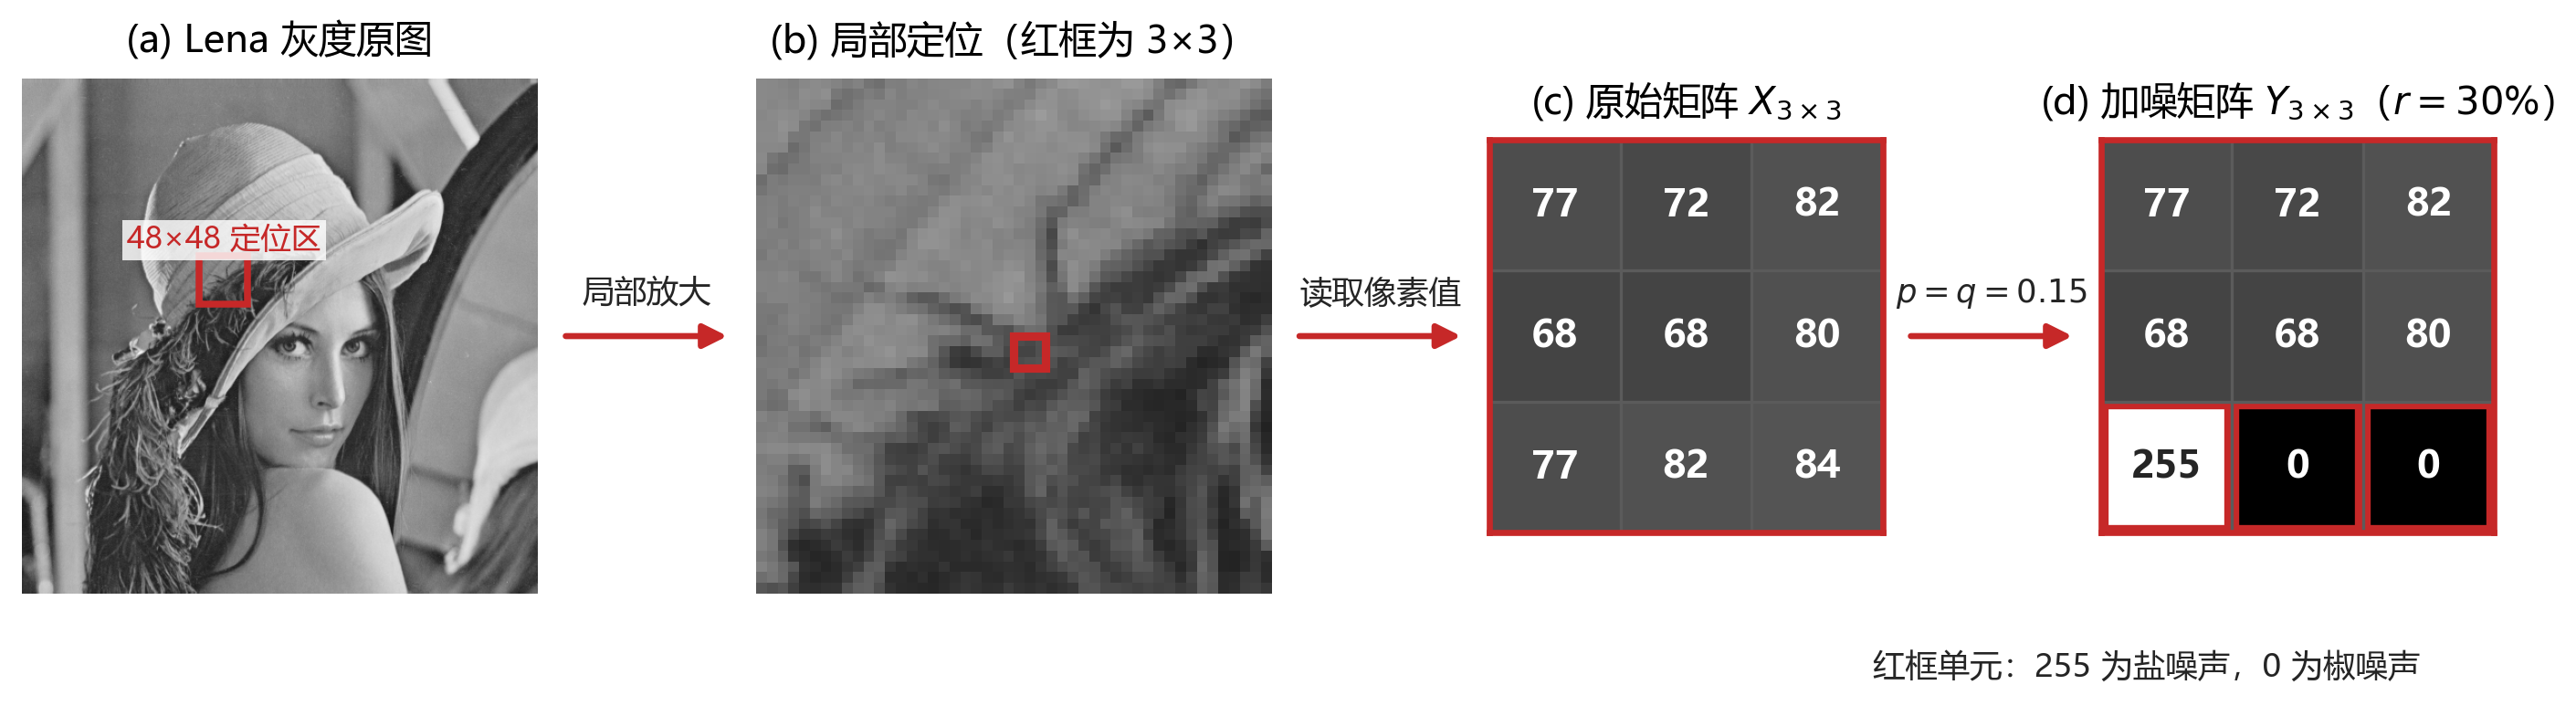
\includegraphics[width=\textwidth]{figures/noise_model_lena_3x3_preview.png}
  \caption{Lena 图像的椒盐噪声生成过程（$r=30\%$）}
  \label{fig:noise_generation}
\end{figure}

由于受污染像素的真实值完全丢失，无法对单个像素单独修复，因此采用两阶段方法：
第一阶段检测出噪声像素的候选集 $\Omega$ 并给出
初值，第二阶段仅在 $\Omega$ 上通过最小化一个保边正则化泛函恢复像素。下面依次
建立两个阶段的模型。

\subsection{第一阶段：自适应中值滤波检测}

中值滤波是最常用的脉冲噪声滤波器：它把每个像素替换为其邻域内像素灰度的中位数。
普通中值滤波对全图统一处理，会在去除噪声的同时损伤细节。自适应中值滤波
（Adaptive Median Filter, AMF）的改进在于两点：其一，只对疑似
噪声像素做替换；其二，当窗口内没有足够的正常灰度层次时自动扩大窗口。

对奇数窗口边长 $w$，记半径 $h=(w-1)/2$，并定义
$S_{i,j}^{w}=\{(k,l):|k-i|\le h,\ |l-j|\le h\}$；当 $(k,l)\notin\mathcal I$ 时，
其灰度值按下文的反射规则由边界内像素补齐。于是 $S_{i,j}^{w}$ 表示中心在 $(i,j)$
的 $w\times w$ 窗口，
$w_{\max}$ 为允许的最大窗口边长。AMF 的判据来自如下观察：若窗口
内同时存在正常的明暗层次，即
\begin{equation}
  s_{\min}^{w}<s_{\mathrm{med}}^{w}<s_{\max}^{w},
\end{equation}
其中 $s_{\min}^{w},s_{\mathrm{med}}^{w},s_{\max}^{w}$ 分别为窗口内灰度的最小值、
中位数与最大值，则窗口信息足以作出判决；否则说明窗口内灰度几乎相同（噪声成片），
需扩大窗口再试。具体流程为：对每个像素依次取 $w=3,5,7,\ldots,w_{\max}$ 逐级检验
上式，直至满足或达到 $w_{\max}$；达到上限仍不满足的像素判为
噪声并用 $w_{\max}$ 窗口的中值替换。对最终窗口，用极值判决
$s_{\min}^{w^*}<y_{i,j}<s_{\max}^{w^*}$ 区分保真像素与噪声像素，其中 $w^*$ 为
该像素停止扩张时的窗口边长。实现中边界像素采用 SciPy \texttt{ndimage} 的
\texttt{reflect} 约定，即反射时重复端点像素；这与 NumPy \texttt{pad} 中同名
模式的端点约定不同。$w_{\max}$ 按噪声等级设定：$30\%$ 取 $7\times7$，
$50\%$ 取 $9\times9$。

\begin{figure}[!htbp]
  \centering
  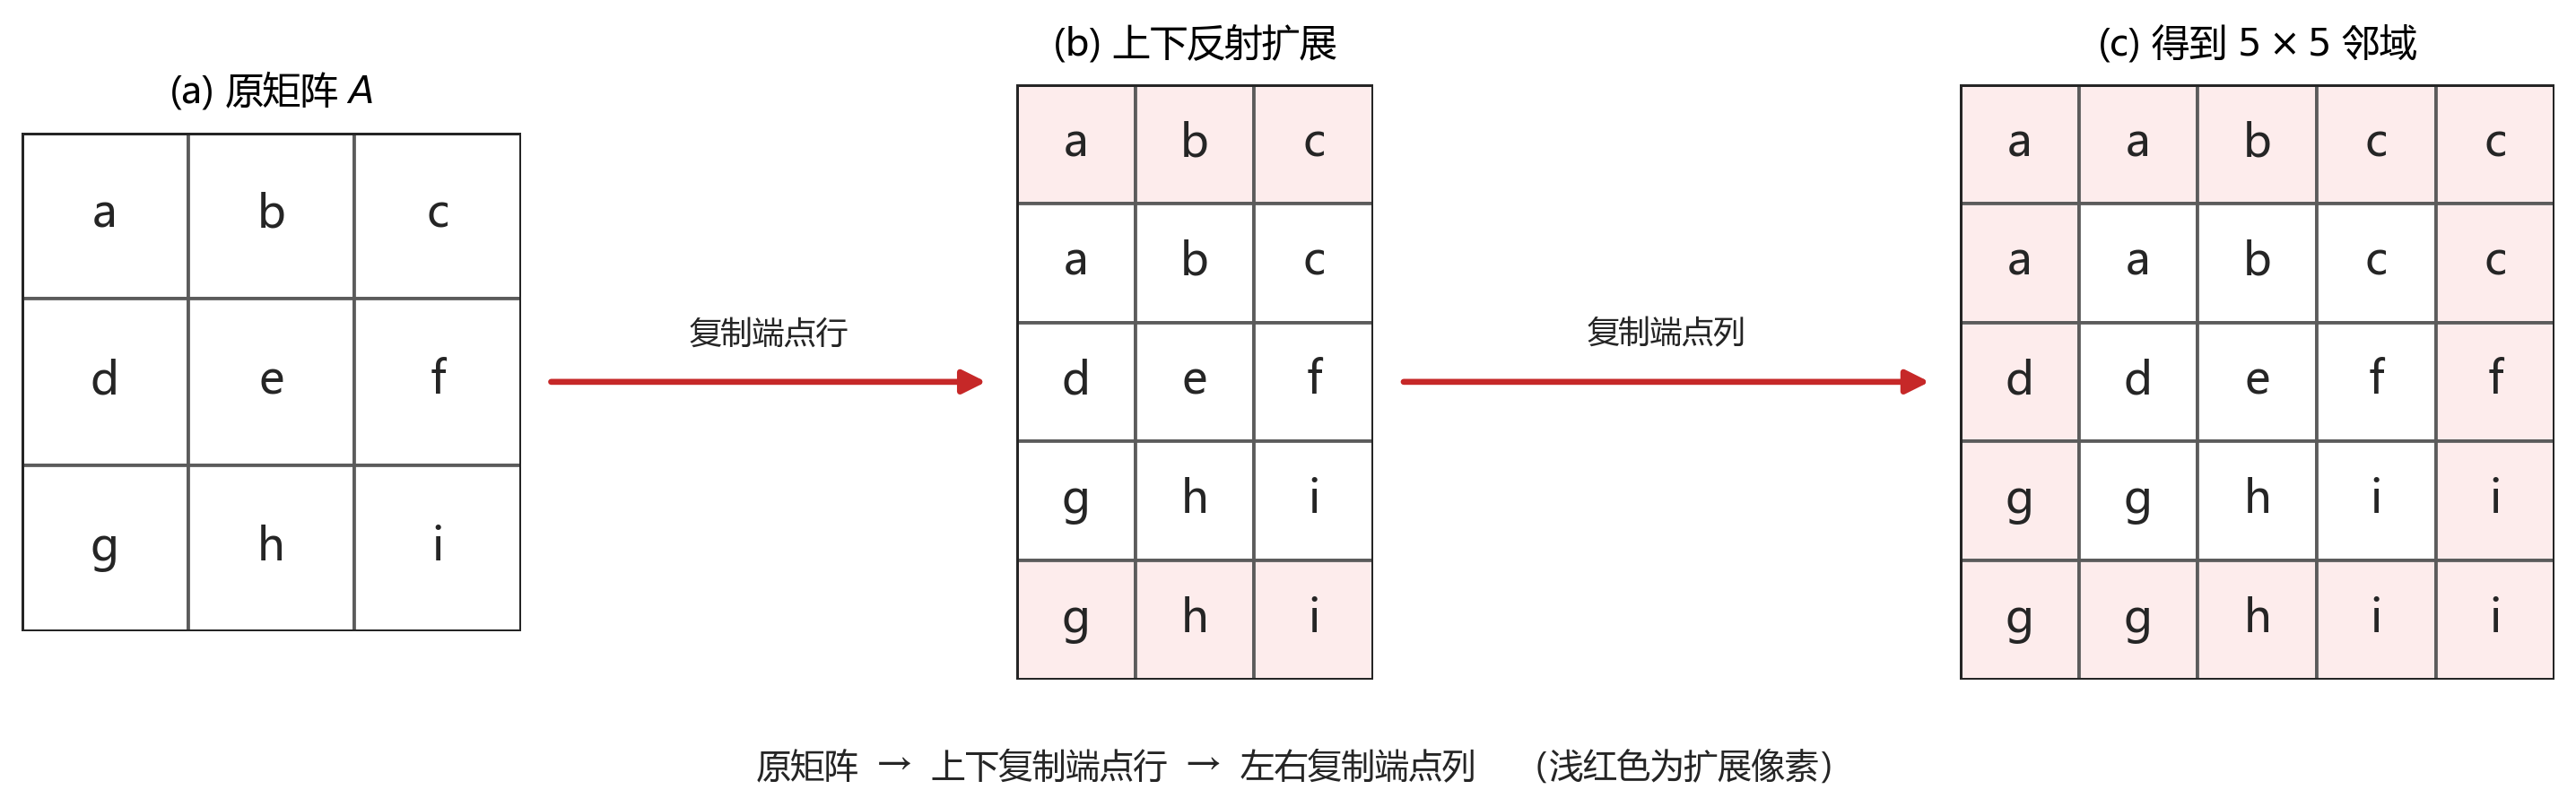
\includegraphics[width=.92\textwidth]{figures/reflect_padding_matrix_preview.png}
  \caption{SciPy \texttt{reflect} 约定下的边界像素扩展示意}
  \label{fig:reflect_padding}
\end{figure}

结合像素端点取值与 AMF 的替换结果，定义噪声候选集为：
\begin{equation}
  \Omega=\big\{(i,j)\in\mathcal I:\ y_{i,j}\in\{s_{\min},s_{\max}\}\ \text{且}\
  \hat y_{i,j}\neq y_{i,j}\big\},
  \label{eq:omega}
\end{equation}
其中 $\hat y_{i,j}$ 为 AMF 的输出。该定义要求候选像素同时满足``取值为动态范围
端点''与``被滤波器替换过''两个条件，可排除两类误判：灰度值恰为端点但被判为
保真的像素没有产生替换，不会进入候选集；非端点像素即使被替换也不满足端点条件。
经验上该定义使误检率由仅用端点判决时的百分之几降至 $1\%$ 以内，是恢复质量提升
的重要来源。

\subsection{第二阶段：保边正则化恢复模型}

第二阶段仅在 $\Omega$ 上恢复像素。为使恢复结果``去噪的同时保留边缘''，需要
引入正则化的思想。图像的边缘指相邻
像素灰度发生跃变的位置，其数学表现是相邻像素差值 $u_p-u_q$ 较大。若用二次
函数惩罚邻域差，则跃变处的代价极高，恢复时会把边缘一并抹平；反之，若惩罚函数
在差值大时仅按线性增长（如 $|t|$），则大差值所受的额外惩罚有限，边缘得以保留。
这类``原点光滑、大尺度处近似线性''的偶凸惩罚函数称为保边势函数，记为
$\varphi_{\alpha}(t)$，$\alpha>0$ 为其参数。问题一主实验取
\begin{equation}
  \varphi_{\alpha}(t)=\sqrt{t^{2}+\alpha},
  \label{eq:phisqrt}
\end{equation}
它处处光滑（$C^{\infty}$），$t=0$ 处二阶导 $\varphi_{\alpha}''(0)=1/\sqrt{\alpha}$
有界，且 $|t|$ 很大时 $\varphi_{\alpha}(t)-|t|\to0$，兼具平滑性与保边性；其余四种
候选势函数在问题二中系统比较。

沿用题目式 (2)，第二阶段的目标函数为
\begin{equation}
  \min_{u}\ \sum_{(i,j)\in\Omega}\Big[|u_{i,j}-y_{i,j}|+\frac{\beta}{2}\big(S_1+S_2\big)\Big],
  \label{eq:p2model}
\end{equation}
其中数据保真项 $|u_{i,j}-y_{i,j}|$ 要求恢复值不远离观测值，
\begin{equation}
  S_1=\sum_{(m,n)\in V_{i,j}\cap\Omega^{C}}2\,\varphi_{\alpha}(u_{i,j}-y_{m,n}),
  \qquad
  S_2=\sum_{(m,n)\in V_{i,j}\cap\Omega}\varphi_{\alpha}(u_{i,j}-u_{m,n}),
\end{equation}
其中 $V_{i,j}=\{(i,j-1),(i,j+1),(i-1,j),(i+1,j)\}\cap\mathcal I$ 为位置
$(i,j)$ 在图像域内的四邻域，
$\Omega^{C}$ 为 $\Omega$ 在 $\mathcal I$ 中的补集。$S_1$ 表示候选像素与干净邻居之间的
正则化约束。由于 $(m,n)\in\Omega^C$，相邻像素保持观测值 $y_{m,n}$；$S_2$ 表示
两个候选像素之间的正则化约束，由于 $(m,n)\in\Omega$，相邻像素同样是待求变量，
因此采用 $u_{m,n}$。又因 $\varphi_\alpha$ 为偶函数，有
$\varphi_\alpha(u-y)=\varphi_\alpha(y-u)$。在式~\eqref{eq:p2model} 的外层求和中，
候选像素--干净像素边只从候选端出现一次，而候选像素--候选像素边会从两个端点
各出现一次。

为进一步看清结构，记 $\tilde u_p=u_p\ (p\in\Omega)$、$\tilde u_p=y_p\
(p\notin\Omega)$，并定义无向边集合
$E_{\Omega}=\{\{p,q\}:q\in V_p,\ \{p,q\}\cap\Omega\neq\varnothing\}$，其中每条
无向边只保留一次。由 $\varphi_{\alpha}$ 的偶性，正则项可等价改写为
\begin{equation}
  F_{\beta}(u)=\sum_{p\in\Omega}|u_p-y_p|+\beta\sum_{\{p,q\}\in E_{\Omega}}
  \varphi_{\alpha}(\tilde u_p-\tilde u_q).
  \label{eq:edgesum}
\end{equation}
对式~\eqref{eq:edgesum} 求梯度，把自身项与来自邻居一侧的贡献合并，并利用
$\varphi_{\alpha}'$ 为奇函数，得
\begin{equation}
  \nabla F_{\beta}(u)_p=\mathrm{sign}(u_p-y_p)+\beta\sum_{q\in V_p}
  \varphi_{\alpha}'(u_p-\tilde u_q).
  \label{eq:grad}
\end{equation}
该式的意义在于：梯度只依赖对每个候选像素的四邻域查值，求和规模与 $|\Omega|$
成正比，不含任何矩阵乘法，为大规模高效求解奠定了基础。

\subsection{光滑化策略}

式~\eqref{eq:grad} 中数据保真项的导数 $\mathrm{sign}(\cdot)$ 在原点不存在，
目标函数非光滑，标准梯度类算法无法直接使用。处理非光滑优化常用两条路线：一是
次梯度类方法，但收敛慢；二是光滑化，即用一族光滑函数
一致逼近非光滑项后求解光滑问题。本文采用后者：选取 $C^1$ 函数 $\rho_{\mu}$
逼近 $|t|$，要求存在与 $t$ 无关的误差界
\begin{equation}
  \big|\rho_{\mu}(t)-|t|\big|\le c_{\rho}\,\mu,\qquad \forall t\in\mathbb{R},
  \label{eq:rhobound}
\end{equation}
其中 $\mu>0$ 为光滑参数，$c_{\rho}$ 为常数。本文实现三种形式，见表~\ref{tab:rho}。

\begin{table}[!htbp]
  \centering\small
  \caption{三种 $\ell_1$ 光滑函数及其逼近误差界}
  \label{tab:rho}
  \begin{tabular}{llc}
    \toprule[1.5pt]
    名称 & $\rho_{\mu}(t)$ & 误差界 \\
    \midrule[1pt]
    平方根型 & $\sqrt{\mu^{2}+t^{2}}$ & $\mu$ \\
    Huber 型 & $\begin{cases}t^{2}/(2\mu), & |t|\le\mu\\ |t|-\mu/2, & |t|>\mu\end{cases}$ & $\mu/2$ \\
    Softplus 型 & $|t|+2\mu\ln(1+e^{-|t|/\mu})$ & $2\mu\ln 2$ \\
    \bottomrule[1.5pt]
  \end{tabular}
\end{table}

主实验取平方根型。以 $\rho_{\mu}$ 替代式~\eqref{eq:edgesum} 中的 $|u_p-y_p|$
即得光滑化模型
\begin{equation}
  \min_{u\in[s_{\min},s_{\max}]^{|\Omega|}}\ F_{\mu}(u)
  =\sum_{p\in\Omega}\rho_{\mu}(u_p-y_p)
  +\beta\sum_{\{p,q\}\in E_{\Omega}}\varphi_{\alpha}(\tilde u_p-\tilde u_q),
  \label{eq:smooth}
\end{equation}
其中光滑化误差满足 $|F_{\mu}(u)-F_{\beta}(u)|\le c_{\rho}\mu|\Omega|$，即
$\mu\to0$ 时目标函数一致收敛到原问题；梯度表达式由式~\eqref{eq:grad} 把
$\mathrm{sign}$ 换成 $\rho_{\mu}'$ 得到。

关于光滑参数 $\mu$ 的选取需要权衡：$\mu$ 越小逼近精度越高，但平方根型
$\rho_{\mu}$ 在原点附近的最大曲率随 $1/\mu$ 增大，而远离原点时曲率迅速减小，
可能使目标函数的条件数变差，从而增加线搜索与迭代的难度；$\mu$ 越大光滑越
充分，但单个数据项的逼近误差上界为 $c_{\rho}\mu$。消融实验表明，
在本文主配置与测试范围内，$\mu$ 从 1 降到 $10^{-4}$ 时迭代数与恢复 PSNR 几乎
不变。因此主实验取 $\mu=1$，此时平方根型逼近的单项误差不超过一个灰度级；
这里的“一致”是数值实验结论，不等同于对 $\mu\to0$ 极限的解析证明。

\subsection{盒约束化与最优性条件}

式~\eqref{eq:smooth} 中的盒约束 $[s_{\min},s_{\max}]$ 引入是无损的，依据最大值原理：当 $\varphi_{\alpha}$ 为偶函数、连续且关于
$|t|$ 严格递增时，目标泛函的任一全局极小点 $u^*$ 必满足
$u_p^{*}\in[s_{\min},s_{\max}]$。其直观解释是：把全部分量逐点截断到动态范围内，
投影的非扩张性保证相邻像素差的绝对值不会增大，且数据项也不会增大。
同时 $\varphi_{\alpha}''\ge0$ 与 $\rho_{\mu}''\ge0$
保证 $F_{\mu}$ 为凸函数，故式~\eqref{eq:smooth} 是盒约束光滑凸规划，其最优性
条件可写为投影残差
\begin{equation}
  G(u)=\big\|P\big(u-\nabla F_{\mu}(u)\big)-u\big\|_{\infty}=0,
\end{equation}
其中 $P(\cdot)$ 为到 $[s_{\min},s_{\max}]$ 的逐像素欧氏投影。$G(u)=0$ 即
一阶 KKT 条件的紧凑表达：在可行域内部梯度为零；在下边界梯度非负，在上边界
梯度非正。
$G(u)$ 同时充当算法的终止准则。

\subsection{算法设计：GPSR-BB 投影梯度法}

GPSR 方法原本用于稀疏重构：以变量分裂把
$\ell_1$ 问题化为有界约束二次规划后，用投影梯度法求解。本文的模型
式~\eqref{eq:smooth} 本身已是盒约束光滑凸问题，可直接沿用其框架。投影梯度法
是约束优化中梯度法的自然推广：每步先沿负梯度方向移动，再投影回可行域。本文
采用其``沿投影弧搜索''的变体：
\begin{equation}
  w^{(k)}=P\big(u^{(k)}-\alpha^{(k)}\nabla F_{\mu}(u^{(k)})\big),\qquad
  u^{(k+1)}=u^{(k)}+\lambda^{(k)}\big(w^{(k)}-u^{(k)}\big),
  \label{eq:pgd}
\end{equation}
即从 $u^{(k)}$ 出发到投影点 $w^{(k)}$ 的线段（投影弧）上搜索新迭代点。

步长 $\alpha^{(k)}$ 取 Barzilai--Borwein（BB）步长：记
$s^{(k)}=u^{(k+1)}-u^{(k)}$、$y^{(k)}=\nabla F(u^{(k+1)})-\nabla F(u^{(k)})$，
先定义候选步长
\[
  \widehat\alpha^{(k+1)}=
  \begin{cases}
    \dfrac{(s^{(k)})^{\!\top}s^{(k)}}{(s^{(k)})^{\!\top}y^{(k)}},
      & (s^{(k)})^{\!\top}y^{(k)}>0,\\[6pt]
    \alpha_{\max}, & (s^{(k)})^{\!\top}y^{(k)}\le0.
  \end{cases}
\]
则截断后的 BB 步长写成分段形式
\begin{equation}
  \alpha^{(k+1)}=
  \begin{cases}
    \alpha_{\min}, & \widehat\alpha^{(k+1)}<\alpha_{\min},\\[2pt]
    \widehat\alpha^{(k+1)}, &
      \alpha_{\min}\le\widehat\alpha^{(k+1)}\le\alpha_{\max},\\[2pt]
    \alpha_{\max}, & \widehat\alpha^{(k+1)}>\alpha_{\max},
  \end{cases}
  \label{eq:bb}
\end{equation}
其中 $[\alpha_{\min},\alpha_{\max}]=[10^{-10},10^{6}]$；曲率信息失效
（$(s^{(k)})^{\!\top}y^{(k)}\le0$）时直接取 $\alpha_{\max}$。BB 步长的思想
是：把相邻两点的差分视为对 Hessian 的割线近似，$\alpha^{(k)}$ 恰为该近似下
$H^{-1}$ 的尺度，从而以极小代价获得近似二阶方法的长步长——这对``不同区域曲率
差异悬殊''的非光滑问题光滑化后尤其有效，是算法效率的关键。

沿弧的步长 $\lambda^{(k)}$ 由非单调 Armijo 条件确定，即取
$\lambda=1,\tau,\tau^{2},\dots$ 中第一个满足
\begin{equation}
  F_{\mu}\big(u^{(k)}+\lambda d^{(k)}\big)\le
  \max_{0\le j\le \min\{M,k\}}F_{\mu}\big(u^{(k-j)}\big)+\delta\lambda(g^{(k)})^{\!\top}d^{(k)}
  \label{eq:armijo}
\end{equation}
者，其中 $d^{(k)}=w^{(k)}-u^{(k)}$，$\delta=10^{-4}$ 为下降系数，$\tau=0.5$
为回溯因子，$M=10$ 为非单调记忆长度。允许目标值在 $M$ 步窗口内暂时上升，可
显著改善 BB 步长波动时的接受率。算法流程见算法 1。

\begin{algtable}{算法 1\quad 两阶段椒盐噪声恢复（GPSR-BB 投影梯度）}
\textbf{输入：}噪声图像 $Y$、噪声等级 $r$、参数 $\alpha,\beta,\mu$、终止容差 tolP \\
\textbf{输出：}恢复图像 $u^{*}$ \\
1: 第一阶段：按 $r$ 查表得 $w_{\max}$，执行 AMF 得候选集 $\Omega$ 与初值
$u^{0}=\hat y|_{\Omega}$ \\
2: 第二阶段：按式~\eqref{eq:smooth} 构造盒约束光滑模型 $F_{\mu}$，
$g^{0}=\nabla F_{\mu}(u^{0})$，
$\alpha^{(0)}=\min\{\alpha_{\max},
\max\{\alpha_{\min},1/\|g^{0}\|_{\infty}\}\}$ \\
3: \textbf{for} $k=0,1,2,\dots$ \textbf{do} \\
\hspace{1.5em} $w^{(k)}=P(u^{(k)}-\alpha^{(k)}g^{(k)})$；\ $d^{(k)}=w^{(k)}-u^{(k)}$ \\
\hspace{1.5em} 求满足式~\eqref{eq:armijo} 的 $\lambda^{(k)}$；
$u^{(k+1)}=u^{(k)}+\lambda^{(k)}d^{(k)}$ \\
\hspace{1.5em} $g^{(k+1)}=\nabla F_{\mu}(u^{(k+1)})$；按式~\eqref{eq:bb} 更新
$\alpha^{(k+1)}$ \\
\hspace{1.5em} \textbf{if} $\|P(u^{(k+1)}-g^{(k+1)})-u^{(k+1)}\|_{\infty}\le$ tolP
\textbf{then} 返回 $u^{*}=u^{(k+1)}$ \\
\textbf{end for}
\end{algtable}

\subsection{参数选择}

正则权重 $\beta$ 与势函数参数 $\alpha$ 对恢复质量有直接影响。由于
$\varphi_{\alpha}=\sqrt{t^{2}+\alpha}$ 关于 $\alpha$ 存在较宽平台，本文在 Lena
图上对 $\beta$ 与 $\alpha$ 做网格扫描（种子 2026）。结果表明：PSNR 随 $\beta$
增大后在 $\beta\ge40$ 时进入平台（$\beta=40$ 时 38.357 dB，提高到 640 仅再提高
0.008 dB）；$\alpha$ 在 300 附近最优，过小则曲率过强、过大则正则过弱。因此主
配置取 $\alpha=300,\ \beta=40$。

\subsection{评价指标}

为评价恢复质量与算法效率，构建如下指标（均在未取整的浮点恢复图 $\hat x$ 上
计算，其中 $\hat x|_{\Omega}=u^{*}$、$\hat x|_{\Omega^{C}}=y$）：
\begin{equation}
  \mathrm{PSNR}=10\log_{10}\frac{(s_{\max}-s_{\min})^{2}}{\mathrm{MSE}},
  \qquad
  \mathrm{SNR}=10\log_{10}\frac{\sum_{i,j}x_{i,j}^{2}}
  {\sum_{i,j}(x_{i,j}-\hat x_{i,j})^{2}},
\end{equation}
其中 $\mathrm{MSE}=\frac{1}{MN}\sum_{i,j}(x_{i,j}-\hat x_{i,j})^{2}$ 为均方误差；
对本文 8 位灰度图，$s_{\max}-s_{\min}=255$。
PSNR 从峰值信号角度度量失真，SNR 从信号能量角度度量噪声水平。另记录平均绝对
误差 $\mathrm{MAE}=\frac{1}{MN}\sum|x-\hat x|$、检测阶段的真噪声检出率
$\mathrm{TPR}$（正确检出的真噪声像素占全部真噪声像素的比例）与误检率
$\mathrm{FPR}$（误判为噪声的干净像素占全部干净像素的比例），以及算法迭代数与
求解时间。

\subsection{求解结果与分析}

本文选取 12 张 $512\times512$ 灰度测试图，在 $30\%$ 和 $50\%$ 两种噪声等级下
分别进行 3 次独立实验，共得到 72 组算例。模型参数取
$\alpha=300,\ \beta=40,\ \mu=1$，求解器参数为 $\delta=10^{-4}$、$\tau=0.5$、
tolP $=10^{-2}$、迭代上限 1500，全部算例均满足终止准则。实验结果见
表~\ref{tab:p1sum}--表~\ref{tab:p1base}，Lena 图像的恢复效果见图~\ref{fig:p1vis}。

\begin{table}[!htbp]
  \centering\small
  \caption{问题一恢复结果汇总}
  \label{tab:p1sum}
  \begin{tabular}{lccccc}
    \toprule[1.5pt]
    噪声等级 & 迭代数 & 时间 s & PSNR dB & SNR dB & 误检率 \\
    \midrule[1pt]
    30\% & 86.8 $[43,204]$ & 2.94 $[1.52,7.08]$ & 37.33 $[30.99,48.17]$ & 31.88 & 0.0\%--0.6\% \\
    50\% & 92.4 $[49,203]$ & 5.42 $[2.93,12.3]$ & 33.76 $[28.29,43.36]$ & 28.31 & 0.0\%--0.7\% \\
    \bottomrule[1.5pt]
  \end{tabular}
\end{table}

\begin{table}[!htbp]
  \centering\small
  \caption{12 张测试图的恢复结果（3 组随机种子均值）}
  \label{tab:p1perimg}
  \begin{tabular}{lcccccc}
    \toprule[1.5pt]
    图像 & 30\% PSNR & 30\% SNR & 30\% 迭代 & 50\% PSNR & 50\% SNR & 50\% 迭代 \\
    \midrule[1pt]
    cameraman & 39.99 & 34.37 & 73 & 35.40 & 29.79 & 81 \\
    house & 48.17 & 43.46 & 44 & 43.36 & 38.65 & 53 \\
    jetplane & 38.20 & 35.36 & 82 & 34.09 & 31.26 & 90 \\
    lake & 34.68 & 29.51 & 173 & 31.10 & 25.93 & 154 \\
    lena & 38.35 & 32.70 & 86 & 34.71 & 29.05 & 94 \\
    livingroom & 34.86 & 28.93 & 88 & 31.17 & 25.23 & 86 \\
    mandril & 33.75 & 28.20 & 61 & 29.72 & 24.16 & 61 \\
    peppers & 37.00 & 31.06 & 86 & 34.18 & 28.24 & 92 \\
    pirate & 35.54 & 29.10 & 105 & 32.16 & 25.71 & 100 \\
    walkbridge & 31.48 & 25.39 & 100 & 28.29 & 22.20 & 98 \\
    woman\_blonde & 30.99 & 25.88 & 86 & 29.21 & 24.10 & 136 \\
    woman\_darkhair & 44.90 & 38.65 & 57 & 41.67 & 35.42 & 65 \\
    \bottomrule[1.5pt]
  \end{tabular}
\end{table}

\begin{table}[!htbp]
  \centering\small
  \caption{不同恢复方法的 PSNR 对比（12 图均值，单位 dB）}
  \label{tab:p1base}
  \begin{tabular}{lccccc}
    \toprule[1.5pt]
    噪声等级 & 噪声图 & 中值滤波 3$\times$3 & 中值滤波 7$\times$7 & AMF 直接输出 & 本文方法 \\
    \midrule[1pt]
    30\% & 10.51 & 23.35 & 26.92 & 32.51 & 37.33 \\
    50\% & 8.28 & 15.10 & 25.66 & 29.13 & 33.76 \\
    \bottomrule[1.5pt]
  \end{tabular}
\end{table}

\begin{figure}[!htbp]
  \centering
  
\includegraphics[width=.92\textwidth]{figures/vis_lena_gray_512_r30.png}
  \caption{Lena 图在 30\% 椒盐噪声下的恢复结果及局部放大}
  \label{fig:p1vis}
\end{figure}

由表~\ref{tab:p1sum} 可知，算法在 $30\%$ 和 $50\%$ 噪声下的平均 PSNR 分别为
37.33 dB 和 33.76 dB，真噪声检出率均不低于 99.8\%，误检率不超过 0.7\%。其中，
Lena 图像在 $30\%$ 噪声下的平均 PSNR 为 38.35 dB。由图~\ref{fig:p1vis} 可见，
恢复图像中的脉冲噪声基本消除，图像边缘和局部纹理得到较好保留。

由表~\ref{tab:p1base} 可知，与固定窗口中值滤波相比，本文方法在两种噪声等级下均
取得更高的 PSNR；在 AMF 直接输出的基础上，平均 PSNR 进一步提高约 4.8--5.1 dB。
算法平均迭代约 87 次和 92 次，求解时间随候选像素数量增加而上升，与复杂度分析一致。

此外，为检验建模中关键选择的必要性，在 Lena 与 Peppers 图上对求解器、光滑参数
与数据保真项做对照实验，结果见表~\ref{tab:p1strategy}。可得三点结论：其一，
BB 步长是求解效率的关键——GPSR-Basic 需 7160 步 266 s，GPSR-BB 仅 85 步
3.19 s，迭代数与时间在三幅对照图上分别降低约 60--88 倍与 50--83 倍，恢复质量
完全相同。其二，光滑参数 $\mu$ 在本配置下由逼近误差决定而非求解效率——消融
实验（存档见支撑材料）显示 $\mu$ 从 1 降到 $10^{-4}$ 时迭代数均为 85 步、恢复
PSNR 差不超过 $0.0001$ dB，$\mu=1$ 是精度与工程便利的双赢选择。其三，数据保真
项在 $\beta$ 足够大时可以删除——无数据项版本 PSNR 为 38.366 dB，比含数据项高
0.009 dB，验证了``第二阶段数据项可删''的论断。

\begin{table}[!htbp]
  \centering\small
  \caption{问题一求解策略对比（Lena 图，$r=30\%$）}
  \label{tab:p1strategy}
  \begin{tabular}{lccc}
    \toprule[1.5pt]
    策略 & 迭代数 & 时间 s & PSNR dB \\
    \midrule[1pt]
    GPSR-Basic 沿投影弧回溯 & 7160 & 265.86 & 38.357 \\
    GPSR-BB 非单调（主配置） & 85 & 3.19 & 38.357 \\
    GPSR-BB BB2 步长 & 79 & 2.96 & 38.357 \\
    GPSR-BB $\mu$ 续延 $(1,10^{-1},10^{-2},10^{-3})$ & 88 & 3.28 & 38.357 \\
    无数据保真项版本 & 97 & 3.69 & 38.366 \\
    \bottomrule[1.5pt]
  \end{tabular}
\end{table}

\section{问题二模型的建立与求解}

\subsection{五种保边势函数及其数学性质}

问题二沿用问题一的两阶段框架，保持噪声检测、数据保真项、邻域结构和求解算法不变，
仅替换正则项中的保边势函数。对第 $k$ 种势函数，将模型中的 $\varphi_\alpha$ 替换为
$\varphi_\alpha^{(k)}$，其余条件保持一致。五种候选势函数为
\begin{align}
  \varphi_{\alpha}^{(1)}(t)&=\sqrt{t^{2}+\alpha},\quad \alpha>0, &
  \varphi_{\alpha}^{(2)}(t)&=|t|^{\alpha},\quad 1<\alpha\le2, \nonumber\\
  \varphi_{\alpha}^{(3)}(t)&=\log\cosh(\alpha t), &
  \varphi_{\alpha}^{(4)}(t)&=\frac{|t|}{\alpha}-\log\Big(1+\frac{|t|}{\alpha}\Big),
  \nonumber\\
  \varphi_{\alpha}^{(5)}(t)&=\begin{cases}\dfrac{t^{2}}{2\alpha}, & |t|\le\alpha,\\[2pt]
  |t|-\dfrac{\alpha}{2}, & |t|>\alpha.\end{cases} & \nonumber
\end{align}

五种势函数均为偶凸函数，并随 $|t|$ 单调增加，其中 $t$ 表示相邻像素的灰度差。
当 $|t|$ 较小时，势函数通过惩罚局部波动抑制噪声；当 $|t|$ 较大时，惩罚增长速度
降低，从而减少对真实边缘的平滑。不同势函数的主要差异体现在原点附近的曲率、远离
原点后的增长速度以及导数是否有界，具体性质见表~\ref{tab:p2smooth}，函数形状见
图~\ref{fig:p2shape}。

\begin{table}[!htbp]
  \centering\small
  \caption{五种势函数的解析性质与光滑化方式}
  \label{tab:p2smooth}
  \begin{tabular}{lccll}
    \toprule[1.5pt]
    势函数 & 光滑类 & 导数界 $|\varphi'|\le$ & 原点二阶导 & 光滑化方式 \\
    \midrule[1pt]
    平方根型 & $C^{\infty}$ & 1 & $1/\sqrt{\alpha}$ & 直接使用 \\
    幂函数型 & $C^{1}$ & 无界 & 奇异 & $(t^{2}+\mu^{2})^{\alpha/2}-\mu^\alpha$ \\
    对数余弦型 & $C^{\infty}$ & $\alpha$ & $\alpha^{2}$ & 直接使用 \\
    对数型 & $C^{2}$ & $1/\alpha$ & $1/\alpha^{2}$ & 直接使用 \\
    Huber 型 & $C^{1}$ & 1 & $1/\alpha$ & 直接使用 \\
    \bottomrule[1.5pt]
  \end{tabular}
\end{table}

\begin{figure}[!htbp]
  \centering
  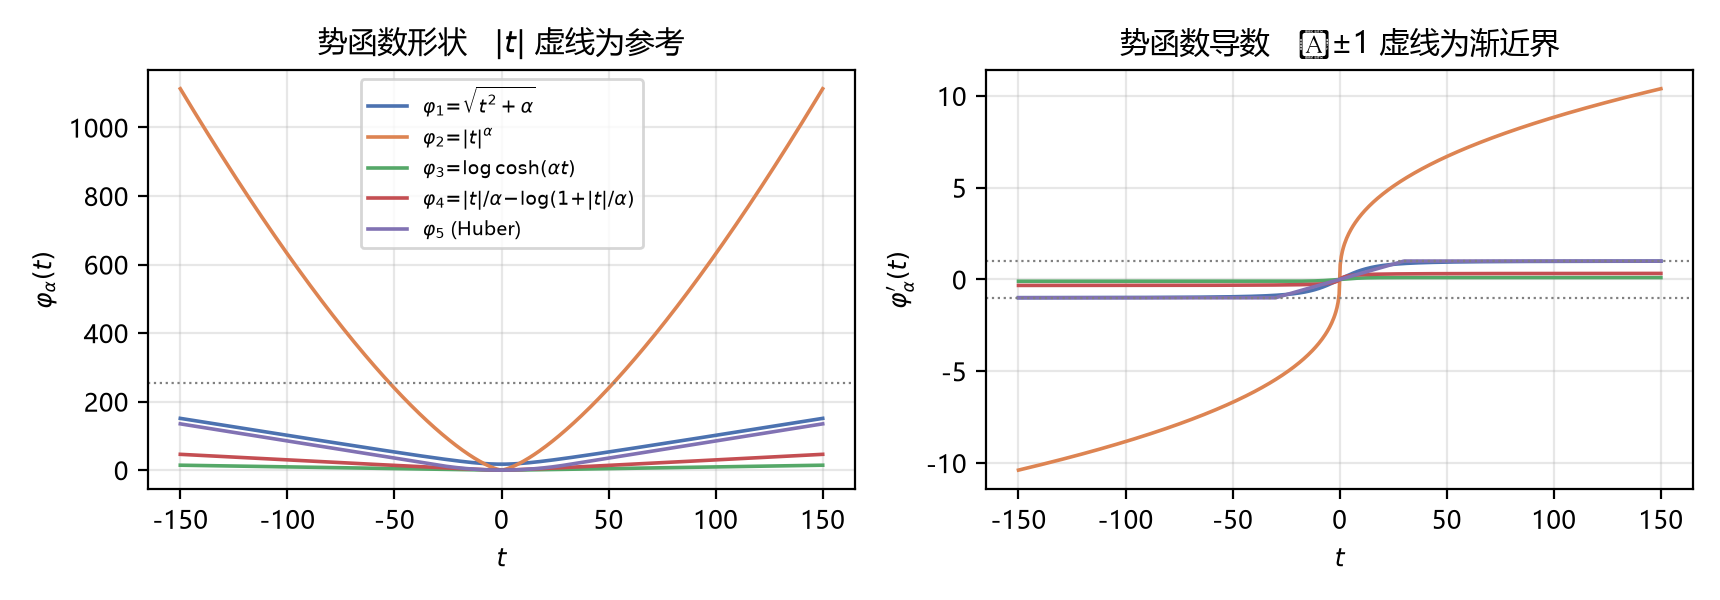
\includegraphics[width=.9\textwidth]{figures/potential_shapes.png}
  \caption{五种保边势函数及其导数曲线}
  \label{fig:p2shape}
\end{figure}

表~\ref{tab:p2smooth} 中的光滑性和导数界直接影响目标函数的曲率，进而影响梯度算法
的稳定性与收敛速度。因此，势函数的比较既要考察恢复质量，也要记录迭代次数。

\subsection{幂函数型的光滑化处理}

当 $1<\alpha<2$ 时，幂函数 $|t|^\alpha$ 在 $t=0$ 附近的二阶导数无界，可能导致
梯度变化过快，降低迭代算法的稳定性。为此，本文采用光滑化处理，
将 $\varphi_{\alpha}^{(2)}$ 近似为
\begin{equation}
  \varphi_{\alpha,\mu}^{(2)}(t)=\big(t^{2}+\mu^{2}\big)^{\alpha/2}-\mu^{\alpha},
\end{equation}
当 $|t|\gg\mu$ 时，该函数与原幂函数近似一致；在 $t=0$ 附近则保持光滑，从而便于
使用梯度算法求解。减去与 $t$ 无关的常数 $\mu^\alpha$ 可保持
$\varphi_{\alpha,\mu}^{(2)}(0)=0$；该常数不改变梯度与极小点，但使不同 $\mu$ 下的
函数值具有一致基准。

\subsection{公平比较协议}

五种势函数中参数 $\alpha$ 的含义不同，若直接使用同一组参数，结果可能主要反映
参数尺度差异，而不能公平反映势函数本身的性能。因此，本文分别标定各势函数的参数：
先固定 $\beta=40$ 搜索 $\alpha$，取该网格内 PSNR 最大的参数记为 $\hat\alpha$；
再固定 $\alpha=\hat\alpha$，搜索 $\beta\in\{5,20,40,80,160,320,640\}$，在满足停止
准则的结果中取该网格内 PSNR 最大者记为 $\hat\beta$。先确定势函数形状，再确定正则项权重，可以减少
参数组合数量，并使各函数在各自较合适的尺度下比较。该过程是一次坐标式标定，
不能保证得到 $\alpha$ 与 $\beta$ 的联合全局最优值；因此本文结论限定在给定网格与
标定协议内。

参数标定使用 Lena 图像及随机种子 2026；参数迁移验证使用其余图像与随机种子，
并在汇总时同时列入 Lena 的标定实例。正式汇总覆盖 Lena、Cameraman 和 Peppers
三幅图像、两个噪声等级及两组随机种子（2026、7）。因此该实验包含样本外的参数
迁移检验，但汇总均值不是完全独立的样本外测试。各方法采用相同的噪声图、停止
准则和最大迭代次数，并使用 PSNR、SSIM 和边缘 PSNR 评价恢复质量，使用迭代次数
评价求解效率。

\subsection{参数敏感性分析}

各势函数的 PSNR 随参数 $\alpha$ 的变化曲线见图~\ref{fig:p2alpha}。

\begin{figure}[!htbp]
  \centering
  
\includegraphics[width=\textwidth]{figures/psnr_vs_alpha.png}
  \caption{五种势函数的参数 $\alpha$ 敏感性}
  \label{fig:p2alpha}
\end{figure}

由图~\ref{fig:p2alpha} 可知，平方根型和 Huber 型在较宽参数区间内保持稳定；对数
余弦型和对数型对参数较为敏感，参数偏离有效区间时 PSNR 明显下降；幂函数经过
光滑化后，其恢复结果随参数变化趋于稳定。因此，参数稳定性也是选择势函数时需要
考虑的因素。

\subsection{对比实验结果与结论}

按标定协议得到各势函数的网格内选定参数后做正式对比，结果见表~\ref{tab:p2main}。

\begin{table}[!htbp]
  \centering\small
  \caption{五种势函数的恢复结果比较}
  \label{tab:p2main}
  \begin{tabular}{llcccccc}
    \toprule[1.5pt]
    $r$ & 势函数 & $\hat\alpha$ & $\hat\beta$ & PSNR dB & SSIM & 边缘 PSNR & 迭代数 \\
    \midrule[1pt]
    30\% & 平方根型 & 300 & 640 & 38.43 & 0.969 & 34.59 & 116 \\
    30\% & 幂函数型 & 1.4 & 640 & 38.39 & 0.969 & 34.56 & 137 \\
    30\% & 对数余弦型 & 0.1 & 640 & 38.29 & 0.969 & 34.44 & 608 \\
    30\% & 对数型 & 3 & 640 & 38.37 & 0.968 & 34.56 & 521 \\
    30\% & Huber 型 & 30 & 640 & 38.24 & 0.969 & 34.36 & 757 \\
    \midrule[1pt]
    50\% & 平方根型 & 1000 & 640 & 34.70 & 0.941 & 30.62 & 53 \\
    50\% & 幂函数型 & 1.6 & 160 & 34.73 & 0.941 & 30.65 & 85 \\
    50\% & 对数余弦型 & 0.1 & 640 & 34.64 & 0.941 & 30.57 & 608 \\
    50\% & 对数型 & 3 & 640 & 34.68 & 0.940 & 30.62 & 611 \\
    50\% & Huber 型 & 30 & 640 & 34.60 & 0.941 & 30.50 & 740 \\
    \bottomrule[1.5pt]
  \end{tabular}
\end{table}

由表~\ref{tab:p2main} 可知，五种势函数在相同噪声等级下的恢复质量接近。$30\%$ 和
$50\%$ 噪声下的 PSNR 极差分别为 0.19 dB 和 0.13 dB，SSIM 及边缘 PSNR 差异较小，
说明在参数适当时，五种势函数均能实现较好的保边恢复。正则权重的敏感性见
图~\ref{fig:p2beta}；多数曲线在 $\beta$ 增大后进入平台或增益逐步收窄，但不同
势函数进入平台的区间并不相同，不能把 $\beta\ge40$ 视为对所有势函数都成立的
统一阈值。

\begin{figure}[!htbp]
  \centering
  
\includegraphics[width=.9\textwidth]{figures/beta_sensitivity.png}
  \caption{五种势函数的正则权重 $\beta$ 敏感性}
  \label{fig:p2beta}
\end{figure}

不同势函数的求解效率差异明显：平方根型和幂函数型约需 50--140 次迭代，对数型、
对数余弦型和 Huber 型约需 500--760 次迭代。综合恢复质量、参数稳定性和求解效率，
本文优先推荐平方根型或经过光滑化处理的幂函数型势函数。

\section{问题三模型的建立与求解}

\subsection{稀疏重构模型与实验实例}

稀疏信号重构是压缩感知的核心问题：信号 $x\in\mathbb{R}^{n}$ 仅含 $s\ll n$ 个
非零元，通过 $m<n$ 个线性观测 $b=Ax+e$ 恢复 $x$，其中
$A\in\mathbb{R}^{m\times n}$ 为测量矩阵，$e$ 为观测噪声。由于方程数少于未知数，
欠定系统 $b=Ax$ 有无穷多组
解；稀疏性是挑选真解的关键先验。直接以``非零元个数最少''为目标即 $\ell_0$
最小化，但该问题是 NP 难的；当 $A$ 满足适当的几何条件（如约束等距性）时，
其凸松弛——$\ell_1$ 正则化最小二乘
\begin{equation}
  \min_{x}\ \tau\|x\|_{1}+\tfrac12\|Ax-b\|_2^{2}
  \label{eq:l1}
\end{equation}
——是常用的可计算凸替代；当测量矩阵满足适当条件时，它可实现精确或稳定的稀疏
恢复，
其中 $\tau>0$ 为平衡数据拟合与稀疏性的正则参数。

实验实例设置为：$n=4096$，$m=1024$，
稀疏度 $s=160$，非零元位置随机且取值为 $\pm1$；$A$ 为行正交化的标准高斯
矩阵；观测 $b=Ax+e$，噪声方差 $\sigma^{2}=10^{-4}$；正则参数取
$\tau=0.1\|A^{\top}b\|_{\infty}$。共生成 10 组独立实例
（种子 0--9）。

\subsection{光滑化与修正 PRP 共轭梯度法}

\subsubsection{共轭梯度法}

共轭梯度法（Conjugate Gradient, CG）是求解大规模优化问题的经典迭代法，只需
存储若干与变量同维的向量，内存开销 $O(n)$。对二次目标函数，共轭梯度法构造的
搜索方向两两关于 Hessian 共轭，理论上不超过 $n$ 步即得精确解。对一般非线性
目标，Polak--Ribière--Polyak（PRP）等共轭参数把这一思想推广为非线性共轭梯度
法：
\begin{equation}
  x_{k+1}=x_k+\alpha_kd_k,\qquad
  d_k=
  \begin{cases}
    -\nabla F_{\mu}(x_0), & k=0,\\
    -\nabla F_{\mu}(x_k)+\beta_k d_{k-1}, & k\ge1,
  \end{cases}
  \label{eq:cgdir}
\end{equation}
其中 $g_k=\nabla F_{\mu}(x_k)$，$\alpha_k$ 由线搜索确定，共轭参数 $\beta_k$
的常见取法有
\begin{equation}
  \beta_k^{\mathrm{FR}}=\frac{\|g_k\|^{2}}{\|g_{k-1}\|^{2}},\quad
  \beta_k^{\mathrm{PRP}}=\frac{g_k^{\top}y_{k-1}}{\|g_{k-1}\|^{2}},\quad
  \beta_k^{\mathrm{HS}}=\frac{g_k^{\top}y_{k-1}}{d_{k-1}^{\top}y_{k-1}},\quad
  \beta_k^{\mathrm{DY}}=\frac{\|g_k\|^{2}}{d_{k-1}^{\top}y_{k-1}},
\end{equation}
其中 $y_{k-1}=g_k-g_{k-1}$ 为相邻梯度差。PRP 参数在精确线搜索下具有``自动
重启''的优良数值性质（某步线搜索充分精确时方向退化为负梯度，相当于重新出发），
但一般线搜索下其全局收敛性无法保证。修正 PRP（PRP+）
以非负截断修正共轭参数：
\begin{equation}
  \beta_k^{\mathrm{PRP}+}=\max\Big\{0,\ \frac{g_k^{\top}y_{k-1}}{\|g_{k-1}\|^{2}}\Big\}.
  \label{eq:prpp}
\end{equation}
截断保证共轭参数恒非负，配合实现中的充分下降性检查与负梯度重启，可避免方向
退化时产生短步甚至停滞，既保留 PRP 数值性能好的特点，又改善异常方向下的稳健性。
相应的全局收敛性需要额外条件：在水平集有界、梯度 Lipschitz 连续、线搜索满足强
Wolfe 条件，且 $\beta_k\ge0$ 并满足 Gilbert--Nocedal 性质 $(*)$ 时，
$\liminf_k\|g_k\|=0$。本文实现的是两项 PRP+ 加下降性重启，相关收敛结论只用于
说明算法成立所需的条件，并不构成对全部工程分支的直接证明。

线搜索采用强 Wolfe 条件：$\alpha_k$ 需同时满足
\begin{equation}
  F_{\mu}(x_k+\alpha_kd_k)\le F_{\mu}(x_k)+c_1\alpha_k g_k^{\top}d_k,
  \qquad
  \big|\nabla F_{\mu}(x_k+\alpha_kd_k)^{\top}d_k\big|\le
  c_2\,\big|g_k^{\top}d_k\big|,
\end{equation}
其中 $c_1=10^{-4}$、$c_2=0.1$。第一式给出充分下降条件，第二式限制新点处方向
导数的绝对值；二者共同排除过短的无效步长和破坏充分下降的过长步长。
实现中另加充分下降保障：若某步方向的下降性不足（$g_k^{\top}d_k\ge
-10^{-7}\|g_k\|^2$）则重置为负梯度方向；强 Wolfe 搜索失败时以负梯度重启与
Armijo 回溯作工程兜底，兜底次数进入诊断计数。需要说明的是，上述收敛结论只
对应强 Wolfe 条件实际成立的迭代，本文不将工程实现笼统表述为无条件全局收敛。

\subsubsection{算法流程}

对模型~\eqref{eq:l1} 的光滑化形式
$F_{\mu}(x)=\tau\sum_i\rho_{\mu}(x_i)+\frac12\|Ax-b\|_2^{2}$，其梯度为
$\tau\rho_{\mu}'(x)+A^{\top}(Ax-b)$。为控制光滑化偏差，$\mu$ 按
$10^{-1},10^{-2},\dots,10^{-6}$ 逐级续延，每段以上一段的解热启动；初值取
$x_0=A^{\top}b$。每段以相邻两步目标相对变化不超过 $10^{-6}$
为主要停止准则，该准则在极小 $\mu$ 段比梯度范数准则更稳健；
同时保留梯度无穷范数不超过 $10^{-6}$ 的提前停止，每段迭代上限 2000。流程见
算法 2。

\begin{algtable}{算法 2\quad 光滑化修正 PRP 共轭梯度法（$\mu$ 续延）}
\textbf{输入：}测量矩阵 $A$、观测 $b$、参数 $\tau$、$\mu$ 序列
$(10^{-1},\dots,10^{-6})$、相对变化容差 rel\_tol \\
\textbf{输出：}重构信号 $x^{*}$ \\
1: $x\leftarrow A^{\top}b$ \\
2: \textbf{for} 每一级 $\mu$（由大到小）\textbf{do} \\
\hspace{1.5em} $g\leftarrow\nabla F_{\mu}(x)$；$d\leftarrow-g$ \\
\hspace{1.5em} \textbf{repeat} \\
\hspace{3em} 强 Wolfe 线搜索求 $\alpha$；$x_{\mathrm{new}}\leftarrow x+\alpha d$；
$g_{\mathrm{new}}\leftarrow\nabla F_{\mu}(x_{\mathrm{new}})$ \\
\hspace{3em} 计算目标相对变化 \\
\hspace{3em} \textbf{if} 目标相对变化 $\le$ rel\_tol \textbf{then}
$x\leftarrow x_{\mathrm{new}}$；$g\leftarrow g_{\mathrm{new}}$；结束本段 \\
\hspace{3em} 按式~\eqref{eq:prpp} 计算 $\beta$；$d\leftarrow-g_{\mathrm{new}}+\beta d$ \\
\hspace{3em} \textbf{if} 下降性不足 \textbf{then} $d\leftarrow-g_{\mathrm{new}}$ \\
\hspace{3em} $x\leftarrow x_{\mathrm{new}}$；$g\leftarrow g_{\mathrm{new}}$ \\
\hspace{1.5em} \textbf{until} 本段终止 \\
\textbf{end for}；返回 $x^{*}=x$
\end{algtable}

\subsection{GPSR-BCQP 对比算法}

GPSR 方法采用变量分裂：把 $x$ 的正部与负部分开，
令 $x=u-v$、$u,v\ge0$，合并为 $z=[u;v]\ge0$，则 $\|x\|_1=\mathbf{1}^{\top}z$，
模型~\eqref{eq:l1} 化为有界约束二次规划（BCQP）
\begin{equation}
  \min_{z\ge0}\ \tfrac12 z^{\top}Bz+c^{\top}z,\qquad
  B=\begin{bmatrix}A^{\top}A&-A^{\top}A\\-A^{\top}A&A^{\top}A\end{bmatrix},\quad
  c=\tau\mathbf{1}+\begin{bmatrix}-A^{\top}b\\ A^{\top}b\end{bmatrix},
\end{equation}
其中 $B$ 为半正定二次型矩阵，$c$ 为线性项。对该二次目标，投影梯度迭代
$w=(z-\alpha\nabla F)_+$、$z\leftarrow z+\lambda(w-z)$ 的弧搜索步长有闭式解
$\lambda=\mathrm{mid}\big(0,\,-g^{\top}s/(s^{\top}Bs),\,1\big)$（二次函数沿弧可
精确最小化），步长 $\alpha$ 取 BB secant 更新，终止准则取
$\|\min(z,\nabla F(z))\|_2\le10^{-3}$。本文实现 GPSR-BB 工程版本，并采用
去偏置过程：固定解的支撑集后做最小二乘
精化，即仅对 $|\hat x_i|$ 显著非零的分量用 $\min\|A_Sx_S-b\|_2$ 重解，以消除
$\ell_1$ 正则对幅度的系统性收缩。

\subsection{求解结果与分析}

10 组独立实例上共对 9 个配置做对比，包括 5 种共轭参数、带续延与不延续的修正
PRP 两种配置、以及 GPSR-BB 与去偏置版本。结果均值见表~\ref{tab:p3main}，收敛
过程与信号恢复对比见图~\ref{fig:p3vis}。

\begin{table}[!htbp]
  \centering\small
  \caption{问题三主实验结果均值，fp 为支撑误报数，真尖峰数 160，续延修正 PRP
  段停止采用相对目标变化准则；GPSR-BB 去偏置行的迭代数含固定支撑最小二乘
  精化 1 步}
  \label{tab:p3main}
  \begin{tabular}{lcccc}
    \toprule[1.5pt]
    方法 & 迭代数 & 时间 s & 相对误差 & fp \\
    \midrule[1pt]
    GPSR-BB & 29.1 & 0.14 & 0.2366 & 8.7 \\
    GPSR-BB 去偏置 & 30.1 & 0.14 & 0.0265 & 2.8 \\
    修正 PRP 单段 & 168 & 2.16 & 0.2444 & 10.9 \\
    原始 PRP 无截断 & 168 & 2.13 & 0.2444 & 10.9 \\
    FR 共轭参数 & 1076 & 20.0 & 0.2428 & 9.8 \\
    HS 共轭参数 & 173 & 2.15 & 0.2437 & 10.3 \\
    DY 共轭参数 & 1084 & 20.4 & 0.2428 & 9.9 \\
    修正 PRP 续延 & 180 & 2.77 & 0.2420 & 10.2 \\
    修正 PRP 续延去偏置 & 180 & 2.77 & 0.0286 & 3.9 \\
    \bottomrule[1.5pt]
  \end{tabular}
\end{table}

\begin{figure}[!htbp]
  \centering
  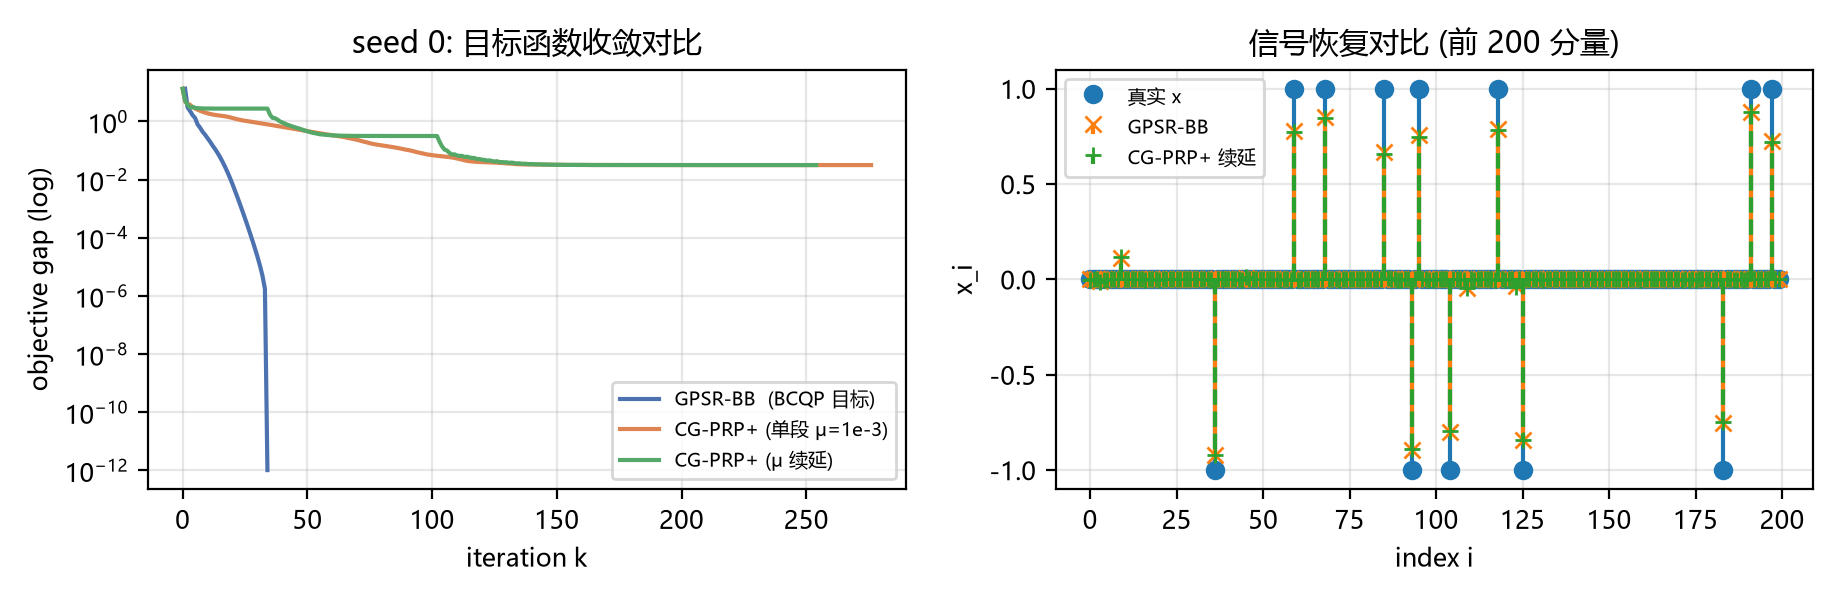
\includegraphics[width=\textwidth]{figures/convergence_signal.png}
  \caption{单实例的目标函数收敛对比与信号恢复对比，左图纵轴为对数尺度}
  \label{fig:p3vis}
\end{figure}

第一，支撑恢复能力。全部方法都恢复出全部 160 个真尖峰；未去偏置时相对误差约
0.24，这是 $\ell_1$ 正则对幅度的系统收缩所致；去偏置后误差
下降约一个数量级：修正 PRP 续延加去偏置与 GPSR-BB 加去偏置的相对误差分别为
0.0286 与 0.0265，支撑误报数 3.9 对 2.8，恢复质量基本持平。这得益于续延把
光滑化偏差从 $\mu=10^{-3}$ 时的 0.50\% 压到 $\mu=10^{-6}$ 时约 0.01\%。

第二，收敛速度。GPSR-BB 以 29 步、0.14 s 收敛，修正 PRP 续延需 180 步、
2.77 s。按``达到相同目标值''口径，GPSR-BB 需 29.1 步 0.14 s，修正 PRP 需
122.7 步 1.64 s，为前者的 4.2 倍。初值与停止准则对共轭梯度法的影响显著：取
零初值并把梯度范数准则用于各段时，同目标值口径需 257.3 步；初值改为
$A^{\top}b$ 并按相对变化准则分段停止后降为 122.7 步，说明初值选择捕获了观测
的主要能量方向，而相对变化准则避免了极小 $\mu$ 段的梯度病态。共轭梯度法的价值
体现在存储量仅 $O(n)$、无需变量分裂与投影，可直接处理问题一、二那样不存在显式
二次型的光滑目标，其速度劣势是``二次结构 + 闭式弧搜索''下的算法匹配性问题。

第三，共轭参数的选择。FR 与 DY 参数需约 1080 步，是修正 PRP 与 HS 参数迭代数
的 6 倍以上，验证了修正 PRP 与 HS 在本组实例上的数值优势。原始 PRP 与修正 PRP
使用相同初值、停止条件、线搜索和下降性保障，仅截断规则不同；两者结果一致，且
诊断记录中负 $\beta$ 和截断次数均为零，说明截断在本组实例上未被触发，
当前实验不能单独证明其数值增益。

\section{灵敏度分析与模型检验}

\subsection{光滑参数的灵敏度}

问题一的消融实验（表~\ref{tab:p1strategy} 与支撑材料存档）显示 $\mu$ 从 1 降到
$10^{-4}$ 时迭代数与恢复 PSNR 均几乎不变，说明该配置下恢复质量与收敛效率对
$\mu$ 均不敏感，$\mu=1$ 的选择由逼近误差决定。问题三的灵敏度方向不同：$\mu$
控制光滑化偏差，$\mu=10^{-3}$ 时 $\ell_1$ 目标值偏差 0.50\%，$\mu=10^{-6}$ 时
降为 0.01\%，而 $\mu=10^{-5}$ 以后线搜索开始退化，说明最优精度存在下界。综合
两题，$\mu$ 的选取应与其控制对象匹配：图像恢复中逼近误差允许达到一个灰度级，
稀疏重构中则需要更精细的控制。

\subsection{正则权重与势函数参数的灵敏度}

问题一的 $\beta$ 网格扫描显示 $\beta\ge40$ 后进入平台。问题二中 $\beta$
扫描上界扩展后，对数型与对数余弦型的选定权重从 160 移至 640，PSNR 分别提升
0.03 dB 与 0.12 dB，说明网格截断会系统性地低估这类势函数的性能。为检验
$\hat\beta$ 落在网格上界 640 是否造成低估，本文在各势函数标定 $\hat\alpha$ 处
补充 $\beta=1280$ 的延伸验证：平方根型、幂函数型、对数型与 Huber 型的 PSNR
增益均不超过 $0.001$ dB，平台结论成立；对数余弦型再提高 $0.046$ dB 与
$0.022$ dB，增量较前一级（$+0.066$ dB 与 $+0.036$ dB）继续收窄、趋于渐近，
即便计入该增益其排序仍不变，验证数据见支撑材料。

\subsection{随机性与实现的鲁棒性}

同一图像同一噪声等级下，三组随机种子（2026、7、42）的 PSNR 标准差为
0.005--0.42 dB，说明算法对噪声的随机实现不敏感。实现层面还需说明两点：其一，
求解器对 BB 步长中曲率信息失效的情况取 $\alpha_{\max}$，并对投影弧
方向做下降性检查，避免数值保护分支造成停滞；其二，梯度与目标函数的求值经过
有限差分校验，问题一三种光滑函数与问题二五种势函数（20 样本）的最大相对误差
均不超过 $6\times10^{-5}$，计算正确性可靠。

\section{模型的评价与推广}

\subsection{模型的优点}

第一，模型链条完整且具有可解释性。本文从噪声模型出发，经两阶段检测、边和形式
的泛函改写、光滑化与盒约束化，逐步建立起可求解的凸规划，每一步都有明确的物理
或数学依据；梯度计算仅依赖四邻域查值，复杂度可控且便于实现。

第二，模型设计中的关键步骤均给出明确的数学定义。检测阶段采用两条件候选集，
把误检率压缩到 $1\%$ 以内；势函数采用光滑函数族与 $\ell_p$ 型光滑处理，
停止准则和初值选择也给出具体实现口径，便于复核模型与计算结果。

第三，实验设计遵循严谨的对比协议。问题一设置了基线方法、求解器、光滑参数与
数据项多个维度的对照，问题二采用独立标定并补充剔除标定图像的样本外汇总，
问题三引入``达到相同目标值''的统一口径，主要评价指标均在多随机种子下汇总，
便于复核结果的稳定性。

\subsection{模型的缺点}

第一，光滑参数 $\mu$ 与正则权重 $\beta$ 的取值依赖实验标定。问题一通过扫描确定
$\mu=1$ 与 $\beta\ge40$ 的合适区间，但缺乏自适应的在线选择准则，对不同类型的
图像或噪声水平可能需要重新标定。

第二，共轭梯度法在小 $\mu$ 段需要靠相对目标变化准则避免梯度病态，该准则的容差
本身需要经验选取，且问题三中其绝对速度明显逊色于 GPSR-BB，反映其适用场景受限。

第三，本文的对比仅覆盖灰度标准图像与单一噪声模型，对彩色图像、随机值噪声与
混合噪声的推广效果尚未验证，结论的外推需谨慎。

\subsection{模型的推广}

第一，两阶段框架可直接推广到随机值噪声与混合噪声场景，只需调整检测阶段的
判决规则，候选集的两条件定义可替换为对应噪声模型的取值特征。

第二，问题二建立的势函数对比协议可推广到其他正则项形式，如总变分、非凸保边
函数，只需补充相应导数与凸性分析。

第三，问题三的光滑化续延策略可用于非负稀疏重构、压缩感知中的其他 $\ell_p$
正则问题，此时只需替换光滑函数族，并沿用相对目标变化的分段停止准则。

\CumcmAIUsed{问题分析与建模思路讨论、代码编写与调试、实验数据核算与文稿语言
润色}

\begin{thebibliography}{10}
  \bibitem[1]{figueiredo2008}
  Figueiredo M A T, Nowak R D, Wright S J. Gradient Projection for Sparse
  Reconstruction: Application to Compressed Sensing and Other Inverse
  Problems[J]. IEEE Journal of Selected Topics in Signal Processing,
  2007, 1(4): 586-597. DOI: 10.1109/JSTSP.2007.910281.
  \bibitem[2]{chan2005}
  Chan R H, Ho C W, Nikolova M. Salt-and-pepper noise removal by
  median-type noise detectors and detail-preserving regularization[J].
  IEEE Transactions on Image Processing, 2005, 14(10): 1479-1485.
  \bibitem[3]{cai2007}
  Cai J F, Chan R H, Fiore C D. Minimization of a Detail-Preserving
  Regularization Functional for Impulse Noise Removal[J]. Journal of
  Mathematical Imaging and Vision, 2007, 29(1): 79-91.
  \bibitem[4]{wu2021}
  Wu C, Wang J, Alcantara J H, et al. Smoothing Strategy Along with
  Conjugate Gradient Algorithm for Signal Reconstruction[J]. Journal of
  Scientific Computing, 2021, 87(21): 1-18. DOI: 10.1007/s10915-021-01440-z.
  \bibitem[5]{liu2025}
  刘莹, 朱志斌, 丁玥宏, 等. Wolfe 线搜索下一个新的共轭梯度法及其在
  信号处理中的应用[J]. 应用数学, 2025, 38(1): 104-113.
  \bibitem[6]{gu2024}
  古恒洋, 杜学武. 一类带有重启步的混合截断谱共轭梯度法及其在图像恢复
  中的应用[J/OL]. 系统科学与数学, 2024. DOI: 10.12341/jssms240367.
  \bibitem[7]{yang2024}
  杨艳雪, 杜守强, 吕施春. 一种新的求解含有 $\ell_1$ 范数优化问题的
  共轭梯度法[J]. 应用数学学报, 2024, 47(4): 643-655.
  \bibitem[8]{narushima2011}
  Narushima Y, Yabe H, Ford J A. A Three-Term Conjugate Gradient Method
  with Sufficient Descent Property for Unconstrained Optimization[J].
  SIAM Journal on Optimization, 2011, 21(1): 212-230.
  \bibitem[9]{chen2010}
  Chen X, Zhou W. Smoothing nonlinear conjugate gradient method for image
  restoration using nonsmooth nonconvex minimization[J]. SIAM Journal on
  Imaging Sciences, 2010, 3(4): 765-790.
  \bibitem[10]{gilbert1992}
  Gilbert J C, Nocedal J. Global convergence properties of conjugate
  gradient methods for optimization[J]. SIAM Journal on Optimization,
  1992, 2(1): 21-42.
\end{thebibliography}

\newpage
\section*{附录一\quad 支撑材料清单}

本文全部程序与结果数据在项目仓库 \texttt{signal-reconstruction/} 中，代码文件
见表~\ref{tab:codemap}，主要结果文件见表~\ref{tab:results}。

\begin{table}[!htbp]
  \centering\small
  \caption{支撑材料：代码文件清单}
  \label{tab:codemap}
  \begin{tabular}{ll}
    \toprule[1.5pt]
    文件 & 功能说明 \\
    \midrule[1pt]
    \texttt{src/noise\_model.py} & 椒盐噪声生成、标准测试图读取 \\
    \texttt{src/amf.py} & 第一阶段自适应中值滤波检测（算法 1 第 1 步） \\
    \texttt{src/restoration\_model.py} & 第二阶段光滑化保边泛函：目标、梯度、5 种势函数 \\
    \texttt{src/solvers.py} & GPSR-Basic / GPSR-BB 投影梯度求解器（算法 1） \\
    \texttt{src/sparse\_reconstruction.py} & 问题三实例生成、光滑化 $\ell_1$ 二次模型 \\
    \texttt{src/cg\_solvers.py} & 非线性共轭梯度（算法 2）与 GPSR-BCQP 对比算法 \\
    \texttt{src/metrics.py} & PSNR / SNR / MAE / SSIM / 边缘 PSNR / 检测统计 \\
    \texttt{exp/problem1/run\_problem1.py} & 问题一主实验（12 图 $\times$ 2 等级 $\times$ 3 种子） \\
    \texttt{exp/problem1/strategy\_compare.py} & 问题一策略对比与 $\mu$ 消融 \\
    \texttt{exp/problem2/tune\_potentials.py} & 问题二 $(\alpha,\beta)$ 独立标定 \\
    \texttt{exp/problem2/verify\_beta1280.py} & 问题二 $\beta=1280$ 网格上界验证 \\
    \texttt{exp/problem2/run\_problem2.py} & 问题二主实验与样本外汇总 \\
    \texttt{exp/problem3/run\_problem3.py} & 问题三 10 实例 9 配置对比实验 \\
    \texttt{exp/problem3/init\_stop\_ablation.py} & 问题三初值与停止准则消融 \\
    \texttt{tests/test\_problem3\_regressions.py} & 回归测试 \\
    \bottomrule[1.5pt]
  \end{tabular}
\end{table}

\begin{table}[!htbp]
  \centering\small
  \caption{支撑材料：主要结果文件清单}
  \label{tab:results}
  \begin{tabular}{ll}
    \toprule[1.5pt]
    文件 & 内容说明 \\
    \midrule[1pt]
    \texttt{exp/problem1/results/tables/problem1\_full.csv} & 问题一 72 算例逐次运行明细 \\
    \texttt{exp/problem1/results/tables/problem1\_summary.csv} & 问题一逐图均值汇总 \\
    \texttt{exp/problem1/results/tables/problem1\_strategy.txt} & 问题一求解器 / $\mu$ / 数据项对照 \\
    \texttt{exp/problem1/results/tables/problem1\_mu\_ablation.csv} & 问题一光滑参数 $\mu$ 消融 \\
    \texttt{exp/problem2/results/tables/problem2\_tuning.txt} & 问题二 $(\alpha,\beta)$ 标定日志 \\
    \texttt{exp/problem2/results/tables/problem2\_summary.csv} & 问题二主实验汇总 \\
    \texttt{exp/problem2/results/tables/problem2\_summary\_oos.csv} & 问题二样本外（剔除 Lena）汇总 \\
    \texttt{exp/problem2/results/tables/problem2\_beta1280\_verification.csv} & $\beta=1280$ 延伸验证 \\
    \texttt{exp/problem3/results/tables/problem3\_full.csv} & 问题三 10 实例逐次明细 \\
    \texttt{exp/problem3/results/tables/problem3\_summary.csv} & 问题三 9 配置均值汇总 \\
    \texttt{exp/problem3/results/tables/problem3\_init\_stop\_ablation.csv} & 初值与停止准则消融 \\
    \bottomrule[1.5pt]
  \end{tabular}
\end{table}

\section*{附录二\quad 主要程序代码}

以下给出四个核心程序（Python 3.11，依赖 NumPy / SciPy），完整代码见支撑材料。

\subsection*{程序 1\quad 自适应中值滤波检测（src/amf.py）}

\begin{lstlisting}[style=appcode]
def adaptive_median_filter(y, r=0.3, wmax=None, s_min=0.0, s_max=255.0):
    """AMF 检测: 逐级扩窗, 返回噪声候选集 cand 与 AMF 输出 y_amf."""
    y = np.asarray(y, dtype=np.float64)
    M, N = y.shape
    if wmax is None:
        wmax = w_max_for_noise_level(r)          # 按噪声等级设定最大窗口
    smin = np.full((M, N), np.nan)               # 各像素最终窗口统计
    smed = np.full((M, N), np.nan)
    smax = np.full((M, N), np.nan)
    active = np.ones((M, N), dtype=bool)         # 尚未确定最终窗口的像素
    for w in range(3, wmax + 1, 2):              # 3,5,7,...,w_max 逐级扩窗
        if not np.any(active):
            break
        # 只在活跃像素的包围盒(外扩 w//2)内计算窗口统计, 结果与全图一致
        idx = np.where(active); pad = w // 2
        i0 = max(int(idx[0].min()) - pad, 0); i1 = min(int(idx[0].max()) + pad + 1, M)
        j0 = max(int(idx[1].min()) - pad, 0); j1 = min(int(idx[1].max()) + pad + 1, N)
        lo, med, hi = _window_stats(y[i0:i1, j0:j1], w, mode="reflect")
        chk_sub = active[i0:i1, j0:j1] & (lo < med) & (med < hi)
        chk = np.zeros((M, N), dtype=bool); chk[i0:i1, j0:j1] = chk_sub
        smin[chk], smed[chk], smax[chk] = lo[chk_sub], med[chk_sub], hi[chk_sub]
        active &= ~chk                           # 满足 smin<smed<smax 即停止扩窗
    if np.any(active):                           # 窗口耗尽: 用 wmax 窗口统计
        lo, med, hi = _window_stats(y, wmax, mode="reflect")
        smin[active], smed[active], smax[active] = lo[active], med[active], hi[active]
    exhausted = active.copy()                    # 从未获得满足窗口的像素
    amf_cand = exhausted | ~((smin < y) & (y < smax))   # AMF 判为噪声的像素
    y_amf = y.copy(); y_amf[amf_cand] = smed[amf_cand]  # 候选像素用中值替换
    # 两条件候选集: y 为端点值且 AMF 输出了替换值
    cand = ((y == s_min) | (y == s_max)) & (y_amf != y)
    return cand, y_amf, dict(smin=smin, smed=smed, smax=smax)
\end{lstlisting}

\subsection*{程序 2\quad 光滑化保边泛函的求值与梯度（src/restoration\_model.py）}

\begin{lstlisting}[style=appcode]
class Phase2Model:
    """光滑化第二阶段模型: F_mu(u) = sum rho(u-y) + beta*sum_edge phi(u_p - u~_q)."""

    def __init__(self, y, mask, beta=5.0, alpha=100.0,
                 smooth="sqrt", potential="sqrt", boundary="reflect"):
        self.y = np.asarray(y, dtype=np.float64)
        self.mask = np.asarray(mask, dtype=bool)          # 候选集 Omega
        self.beta, self.alpha = float(beta), float(alpha)
        self.phi, self.dphi, self.phi_sm, self.dphi_sm = POTENTIALS[potential]
        self.rho, self.drho = SMOOTHINGS[smooth]
        self.mu, self.with_data = 1.0, True
        self.nvars = int(np.sum(self.mask))
        self.idx_map = np.full(self.mask.shape, -1, dtype=np.int64)
        self.idx_map[self.mask] = np.arange(self.nvars, dtype=np.int64)
        self.coords = np.argwhere(self.mask)
        self._build_topology()                            # 预计算四邻域索引表

    def value(self, u):                                   # 目标函数 F_mu(u)
        u = np.asarray(u, dtype=np.float64)
        yN = self.y[self.mask]
        fdata = np.sum(self.rho(u - yN, self.mu)) if self.with_data else 0.0
        freg = 0.0
        for d in range(self.ndirs):                       # 4 个邻域方向
            k = self.nb_kind[d]
            m0 = np.where(k == 0)[0]                      # 邻居为干净像素: 2*phi
            if m0.size:
                freg += 2.0 * np.sum(self.phi_sm(u[m0] - self.nb_yval[d][m0],
                                                 self.alpha, self.mu))
            m1 = np.where(k == 1)[0]                      # 邻居为候选变量: phi
            if m1.size:
                freg += np.sum(self.phi_sm(u[m1] - u[self.nb_idx[d][m1]],
                                           self.alpha, self.mu))
        return fdata + 0.5 * self.beta * freg

    def gradient(self, u):                                # 梯度(四邻域查值)
        u = np.asarray(u, dtype=np.float64)
        yN = self.y[self.mask]
        g = self.drho(u - yN, self.mu) if self.with_data else np.zeros_like(u)
        for d in range(self.ndirs):
            k = self.nb_kind[d]
            m0 = np.where(k == 0)[0]
            if m0.size:
                g[m0] += self.beta * self.dphi_sm(u[m0] - self.nb_yval[d][m0],
                                                  self.alpha, self.mu)
            m1 = np.where(k == 1)[0]
            if m1.size:
                g[m1] += self.beta * self.dphi_sm(u[m1] - u[self.nb_idx[d][m1]],
                                                  self.alpha, self.mu)
        return g
\end{lstlisting}

\subsection*{程序 3\quad GPSR-BB 投影梯度求解器（src/solvers.py）}

\begin{lstlisting}[style=appcode]
def gpsr_bb(model, u0, mu=1e-3, lo=0.0, hi=255.0, tolP=1e-2, tolX=1e-10,
            maxit=5000, amin=1e-10, amax=1e6, delta=1e-4, tau=0.5,
            lsearch_max=30, M=10, bb_variant=1):
    """BB 步长 + 投影 + 非单调 Armijo 线搜索 (算法 1)."""
    model._set_mu(mu)
    z = np.asarray(u0, dtype=np.float64).copy()
    g = model.gradient(z)
    a0 = 1.0 / max(1.0, float(np.max(np.abs(g))))
    a = float(min(amax, max(amin, a0)))
    hist_f = [model.value(z)]; hist_gap = [projection_gap(z, g, lo, hi)]
    converged = False
    for it in range(1, maxit + 1):
        w = project(z - a * g, lo, hi)                    # 投影点
        d = w - z                                         # 投影弧方向
        gd = float(np.dot(g, d))
        fref = max(hist_f[-min(M, len(hist_f)):])         # 非单调参考值
        lam, accepted = 1.0, False
        for _ in range(lsearch_max):                      # 回溯搜索 lam
            fnew = model.value(z + lam * d)
            if fnew <= fref + delta * lam * gd:           # 非单调 Armijo 条件
                accepted = True
                break
            lam *= tau
        if not accepted:                                  # 兜底: 最速下降方向重试
            d = -g / max(1.0, float(np.linalg.norm(g))); gd = float(np.dot(g, d))
            lam, accepted = 1.0, False
            for _ in range(lsearch_max):
                fnew = model.value(z + lam * d)
                if fnew <= fref + delta * lam * gd:
                    accepted = True
                    break
                lam *= tau
            if not accepted:
                break
        z_new = z + lam * d
        g_new = model.gradient(z_new)
        s, y_ = z_new - z, g_new - g
        if float(np.linalg.norm(s)) > 1e-14:
            a = bb_stepsize(s, y_, amin, amax, variant=bb_variant)   # BB 步长
        z, g = z_new, g_new
        hist_f.append(model.value(z)); hist_gap.append(projection_gap(z, g, lo, hi))
        if hist_gap[-1] <= tolP or float(np.max(np.abs(s))) <= tolX:
            converged = True                              # 投影间隙 <= tolP: KKT
            break
    return dict(u=z, it=it, hist_f=np.array(hist_f), hist_gap=np.array(hist_gap),
                converged=bool(converged))
\end{lstlisting}

\subsection*{程序 4\quad 修正 PRP+ 共轭梯度法（src/cg\_solvers.py）}

\begin{lstlisting}[style=appcode]
def nonlinear_cg(model, x0, beta="prp+", maxit=5000, tolG=1e-6, c1=1e-4, c2=0.1,
                 stop="rel", rel_tol=1e-6, safeguard=True, fallback=True):
    """非线性共轭梯度 (强 Wolfe 线搜索), stop='rel' 为相对目标变化停止准则."""
    x = np.asarray(x0, dtype=np.float64).copy()
    g = model.gradient(x)
    d = -g.copy()
    f_cur = model.value(x)
    counts = dict(negative_beta_count=0, beta_truncation_count=0,
                  descent_restart_count=0, line_search_fallback_count=0)
    it = 0
    for it in range(1, maxit + 1):
        if float(np.max(np.abs(g))) <= tolG:              # 梯度准则提前停止
            break
        alpha, ls_failed = strong_wolfe_alpha(model, x, d, g, c1, c2)
        counts["line_search_fallback_count"] += int(ls_failed)
        if alpha <= 0.0 or ls_failed:                     # 兜底: 负梯度重试
            if not fallback:
                break
            d = -g.copy()
            alpha, ls_failed = strong_wolfe_alpha(model, x, d, g, c1, c2)
            counts["line_search_fallback_count"] += int(ls_failed)
            if alpha <= 0.0:
                break
        x_new = x + alpha * d
        g_new = model.gradient(x_new)
        f_new = model.value(x_new)
        if stop == "rel" and it > 1:                      # 相对目标变化停止
            if abs(f_new - f_cur) / max(abs(f_cur), 1e-12) <= rel_tol:
                x, g, f_cur = x_new, g_new, f_new
                break
        y_prev = g_new - g
        if beta in ("prp", "prp+"):                       # beta = g'y / g'g
            den = float(np.dot(g, g))
            raw_beta = float(np.dot(g_new, y_prev)) / den if den > 1e-300 else 0.0
        elif beta == "hs+":                               # HS 参数
            den = float(np.dot(d, y_prev))
            raw_beta = float(np.dot(g_new, y_prev)) / den if abs(den) > 1e-300 else 0.0
        else:                                             # FR / DY
            raw_beta = None
        if raw_beta is not None and raw_beta < 0.0:       # 诊断: 负 beta / 截断
            counts["negative_beta_count"] += 1
            if beta in ("prp+", "hs+"):
                counts["beta_truncation_count"] += 1
        b = beta_rule(beta, g_new, g, d, y_prev)
        d_new = -g_new + b * d
        gd = float(np.dot(g_new, d_new))
        if safeguard and gd >= -1e-7 * float(np.dot(g_new, g_new)):
            d_new = -g_new.copy()                         # 下降性不足: 重启
            counts["descent_restart_count"] += 1
        x, g, d, f_cur = x_new, g_new, d_new, f_new
    return dict(x=x, it=it, conv=True, **counts)

def cg_with_mu_continuation(model, x0, mu_seq=(1e-1, 1e-2, 1e-3),
                            beta="prp+", maxit=2000, tolG=1e-6,
                            stop="rel", rel_tol=1e-6, safeguard=True):
    """mu 续延: 由大到小逐段求解, 每段以上一段解热启动 (算法 2)."""
    x = np.asarray(x0, dtype=np.float64).copy()
    it_sum, it_hist, conv_all = 0, [], True
    for mu in mu_seq:
        model.set_mu(float(mu))
        res = nonlinear_cg(model, x, beta=beta, maxit=maxit, tolG=tolG,
                           stop=stop, rel_tol=rel_tol, safeguard=safeguard)
        x = res["x"]; it_sum += int(res["it"]); it_hist.append(int(res["it"]))
        conv_all &= bool(res["conv"])
    return dict(x=x, it_sum=it_sum, it_hist=it_hist, conv=conv_all)
\end{lstlisting}

\end{document}
